\documentclass[12pt,a4paper]{book}
\usepackage{amsmath}
\usepackage{amssymb}
\usepackage{listings}
\usepackage{amsfonts}
\usepackage{tabulary}
\usepackage{graphicx}
\usepackage[dvipsnames]{xcolor}
\usepackage{algorithm}
\usepackage[noend]{algpseudocode}
\usepackage[margin=1in]{geometry}
\usepackage{todonotes}
\usepackage{msc}
\usepackage{datetime}
\setmsckeyword{}
\drawframe{no}% switch of msc frame
\usepackage{tikz}
\usepackage{skak}
\usepackage[T1]{fontenc}
\usetikzlibrary{matrix,chains,positioning,decorations.pathreplacing,arrows}


\setcounter{tocdepth}{3}
\usepackage{enumitem}
\usepackage{url}

\newcommand{\TT}[1]{\texttt{#1}}

\renewcommand{\baselinestretch}{1.1} 



\newenvironment{absolutelynopagebreak}
{\par\nobreak\vfil\penalty0\vfilneg
  \vtop\bgroup}
{\par\xdef\tpd{\the\prevdepth}\egroup
  \prevdepth=\tpd}


\makeatletter
\newcommand{\@giventhatstar}[2]{\left(#1\;\middle|\;#2\right)}
\newcommand{\@giventhatnostar}[3][]{#1(#2\;#1|\;#3#1)}
\newcommand{\giventhat}{\@ifstar\@giventhatstar\@giventhatnostar}
\makeatother

\graphicspath{{graphs/}}

\title{Deep Reinforcement Learning for Chess}
\date{\today}
\author{Computer Science Tripos, Part II}


\begin{document}

\pagestyle{empty}

\hfill{\LARGE David Yu-Tung Hui}

\vspace*{80mm}
\begin{center}
\LARGE
{Deep Reinforcement Learning for Chess} \\
\large
\vspace*{10mm}
Computer Science Tripos, Part II \\
\vspace*{5mm}
Trinity College \\
\vspace*{5mm}
\today
\end{center}

\cleardoublepage


\setcounter{page}{1}
\pagenumbering{roman}
\pagestyle{plain}


\chapter*{Proforma}

{\large
  \begin{tabular}{ll}
    Name:               & \bf David Yu-Tung Hui\\
    College:            & \bf Trinity College\\
    Project Title:      & \bf Deep Reinforcement Learning for Chess\\
    Examination:        & \bf Computer Science Tripos, Part II, July 2018\\
    Word Count:         & \bf 11990 \footnotemark[1]\\
    Project Originator: & David Yu-Tung Hui\\
    Supervisor:         & Dr. Sean Holden\\ 
  \end{tabular}
}
\footnotetext[1]{According to TurnItIn for dyth2\_dissertation1. TeXCount 3.1, excluding reference numbers, pictures, headers and footers, gives a wordcount of 10022}

\stepcounter{footnote}


\section*{Original Aims of the Project}

\paragraph{} To create and train a chess agent using deep reinforcement learning. Within a game of 80 plys, the agent would be stronger than an agent playing random moves to 95 \% significance. The goal of the project was to modify Giraffe, an existing chess engine, to utilise a neural network written in the \texttt{Python} deep learning package \texttt{PyTorch}. The resulting chess engine would then be trained by self-play using reinforcement learning algorithms.

\section*{Work Completed}

\paragraph{} A chess agent was implemented and sufficiently trained to fulfill the objective. As it was easier to modify Stockfish instead of Giraffe, the final codebase used a search algorithm based on Stockfish which utilised a neural network written in \texttt{PyTorch}. A novel neural network architecture and board representation was created, reducing the amount of human information used in training to be below the majority of published techniques.

\section*{Special Difficulties}

\paragraph{} The most difficult part of the project was in finding good hyperparameter values which enabled convergence of the reinforcement learning algorithms to be numerically stable. This problem was exacerbated by long training times of the chess engine, which could take up to several days. Implementation of temporal difference learning was not straightforward because its equations had been incorrectly written by some sources.

\newpage
\section*{Declaration}

I, David Hui of Trinity College, being a candidate for Part II of the Computer Science Tripos, hereby declare that this dissertation and the work described in it are my own work, unaided except as may be specified below, and that the dissertation does not contain material that has already been used to any substantial extent for a comparable purpose.

\bigskip
\leftline{Signed:}

\medskip
\leftline{Date: \today}

\cleardoublepage

\tableofcontents

%\listoffigures

\newpage
\section*{Acknowledgements}

\paragraph{} First, I would like to thank my supervisor and Director of Studies, Dr. Sean Holden, for his advice, feedback and help over the past eight months. His advice on the direction of implementation, and feedback on the dissertation writeup was invaluable.

\paragraph{} I am grateful to Petar Veli\v ckovi\' c for allowing me access to a research machine from the Computational Biology Group, and for his assistance in the project proposal and progress presentation.

\paragraph{} Finally, I am indebted to my parents for their constant support, encouragement and advice throughout the course of this project, and throughout my journey in life.

\cleardoublepage

\setcounter{page}{1}
\pagenumbering{arabic}
\pagestyle{headings}






\chapter{Introduction}

\paragraph{} This project analyses a chess engine trained by self-play. A chess engine simulates moves with a search algorithm and predicts their chances of winning using an evaluation function. This function was approximated with a neural network and trained by deep reinforcement learning. The neural network, search and learning algorithms were implemented in \texttt{C++} and \texttt{Python}, interfacing with components from Stockfish. Within a chess game of 80 plys, agents trained with TD($\lambda$) and TD-Leaf($\lambda$) were sigificantly stronger than an opponent playing random moves to 95\% confidence, fulfilling the success criteria. Overall, the project demonstrates that deep reinforcement learning can train an agent to discover strategies and subgoals from first principles, without the need for human knowledge or interference.

\section{Motivation}

\paragraph{} The dream of Artificial Intelligence (AI) has been described as ``our last invention'' \cite{ailast}. Capable of empowering, befriending or destroying humanity, this subfield of Computer Science has been prominent in media and popular culture. However, many AI architectures are not currently deployed in the overwhelming complicated natural world. Instead, their capabilities are evaluated in artificial environments such as chess.

\paragraph{} Chess is ideal for evaluation because it is small enough to simulate but not trivially small. Its size is determined by its branching factor, the average number of possible next states. In chess, this number is around 20. Because of this property, research from figures such as Alan Turing, Claude Shannon, IBM and Google DeepMind has developed chess playing agents, or engines, of increasing strength \cite{michieIntel} \cite{shannonlegendary} \cite{deepBlue} \cite{alphazero}. Nowadays, chess engines of superhuman ability can be found on ubiquitous commercial hardware.

\paragraph{} Early chess engines use knowledge engineering algorithms. They relied on hand-crafted evaluation functions which could take years to develop. \cite{stockfish} These cannot be transferred to other games and may even be suboptimal. To resolve these issues, agents should reduce their dependency on human information and bias by learning from its surrounding environment. By augmenting the environment with a reward signal, reinforcement learning trains an agent to discover strategies and subgoals. Through exploration, an agent learns to maximise the reward, or payoff, obtained when goals are met. \cite{Sutton} In chess, wins are rewarded positively and losses negatively, enabling an agent to learn from successes and mistakes. The agent is trained by self-play, because the ideal opponent when learning is one of equal strength. \cite{ban}
% BAN 2012 SELF PLAY GOOD

\paragraph{} Recent achievements in machine learning have been due to the subfield of deep learning. Deep learning algorithms train a neural network to approximate functions by inferring representations from a dataset. \cite{deeplearn} By training a neural network to approximate an evaluation function with reinforcement learning, a chess agent can be trained by deep reinforcement learning. \cite{AlphaGo} \cite{DQN}

\paragraph{} The aim of this project was to train a chess engine using deep reinforcement learning such that the difference in strength between it and an opponent playing random moves is statistically significant to 95 \%. Such an agent could be evaluated not just against knowledge engineering or machine learning agents, but against the many centuries of human chess knowledge. A chess engine trained with minimal human knowledge would not only create a new opponent, but may contribute new knowledge to chess.

% why random agent is good
\paragraph{} The only way of determining that the agent has been successfully trained is by playing against an opponent which moves randomly. As the agent is trained by self-play, and it gets stronger with every game, the agent is more likely to perform better against strong opponents, rather than against any opponent. To ensure that the agent can play against all opponents, it should be play against an agent generating random moves, capable of emulating an opponent of any strength. As the average length of a game of chess is 80, it was chosen as an upper bound on the length of a game of chess.

\section{Related Work}

\paragraph{} One of the earliest reinforcement learning chess engines is KnightCap. The evaluation function was a linear combination trained using TD-Leaf($\lambda$) against humans. After 300 games, KnightCap was as strong as a human master. \cite{knightcap}

\paragraph{} Giraffe was developed in 2015 and is similar to this project. It is one of the first agents to be trained using deep reinforcement learning. The evaluation function was a four layer neural network trained by a variant of TD-Leaf($\lambda$). After 50000 games of self-play, Giraffe reached the standard of an international master. \cite{giraffe}

\chapter{Preparation}

\paragraph{} A literature review of three chess engines and three reinforcement learning algorithms was performed in order to refine the plan in the project proposal. All of the engines examined had open-source codebases. The chess engines Giraffe, Stockfish and Sunfish were examined. Reinforcement learning algorithms were investigated using their codebase and the papers of Giraffe, the chess engine KnightCap and the backgammon agent TD-Gammon. A summary of findings is duly presented, as well as the refined plan.

%\paragraph{} Understanding of chess is not integral to understanding this project. The reader is assumed to have no prior knowledge of chess, apart from knowing that chess is a finite, discrete and deterministic game. A chess game has a finite number of moves and always terminates without relying on chance. Players take discrete turns to move pieces around a chessboard consisting of 8 by 8 discrete squares. It is not an option to skip a turn: players must move a piece or forfeit the game. Finally, a chess game always ends in checkmate or draw.

\section{Components of a Chess Engine}

% shannon algorithms
\paragraph{} A rational chess engine plays to maximise its probability of winning. It selects moves with a search algorithm simulating all possible games and outcomes from the current chessboard position. The best move leads to the greatest proportion of positive outcomes. Unfortunately, this strategy is infeasible for chess because there are too many outcomes to search. Chess lasts 10 minutes, so each player has a total of 5 minutes thinking time. An average game has $10 ^{120}$ outcomes and 80 moves, known as plys. The average thinking time for each ply is less than 5 seconds, an unreasonably short time to simulate all outcomes. To reduce computation, a heuristic called an evaluation function approximates the probability of winning given a board position. Instead of simulating to conclusion, a search algorithm uses this heuristic after a simulating a few plys.

% move generator
\paragraph{} The strength of a chess engine depends on the speed of its search algorithm and the accuracy of its evaluation function. The evaluation function in this project is a neural network. It is trained by deep reinforcement learning, a process which trains the neural network from its experience of playing games. The most important component of the project is the search algorithm, because it is thus used in training as well as playing. Its speed is bottlenecked by its move generator, a function which the search algorithm is built around. This function is called for every move and returns a list of legal moves, enabling all possible games to be simulated. The project adapted move generators from open-source chess engines due to the complexity of reimplementing and optimising another.

\section{Search Algorithms}

\paragraph{} Minimax was the first search algorithm to utilise an evaluation function. Since its publication in 1950 by Claude Shannon, it is used by the majority of chess agents. \cite{shannonlegendary} In 1959, John McCarthy improved Minimax using an alpha-beta pruning heuristic. This recognised that further evaluations of a move were unnecessary if a better alternative had already been found. This could be further improved by ordering the moves such that they were pruned as often as possible. A turning point in computer chess occurred in 1967, when Richard Greenblatt used a transposition table to cache chessboard positions and scores. His agent, Mac Hack IV, became the first chess engine to defeat a human. \cite{russellNorvig} Since then, increasingly advanced and specific heuristics have been developed. These were not implemented because they are empirically derived from human bias and may limit the teaching ability of reinforcement learning.

\subsection{Minimax Searching Algorithm}

\paragraph{} Minimax is a portmanteau of minimise and maximise, two functions which compose its operation. Minimax is applied to two player zero-sum games like chess, where one player's payoff or reward is negated from the other. As a rational player maximises potential payoff, this minimises their opponent's potential payoff. By assuming that the opponent is also rational, Minimax finds moves by recursively maximising what their opponent has minimised. This algorithm has a complexity of $\mathcal{O}(b^d)$. \cite{carolus} An efficient way of implementing this is Negamax, Algorithm \ref{Negamax}.

\begin{algorithm}
  \caption{Negamax}\label{Negamax}
  This implementation searches to depth $depth$ from root position $position$, returning the best move and its score. The function should be called by \Call{Negamax}{$position, depth-1$}.
  \begin{algorithmic}[1]
    \Function{Negamax} {$position, depth$}
    \If {$depth = 0$ or $\Call{noFurtherPossibleMoves}$}
    \State \textbf{return} $\_, \Call{evaluate}{position}$
    \EndIf
    \State $max \gets -\infty$
    \State $maxMove$
    \For {$move$ in \Call{moveGenerator}{$position$}}
    \State \Call{doMove}{$position, move$}
    \State $score \gets -\Call{Negamax}{position, depth-1}[1]$
    \State \Call{undoMove}{$position, move$}
    \If {$score \geqslant max$}
    \State $max \gets score$
    \State $maxMove \gets move$
	\EndIf
    \EndFor
    \State \textbf{return} $maxMove, max$
    \EndFunction
  \end{algorithmic}
\end{algorithm}

\paragraph{} In Game Theory, Minimax finds a Nash equilibrium. This is a state of play where changing strategies leads to suboptimal outcomes if their opponent does not change strategies. Hence Minimax should be used to find moves throughout a match. \cite{russellNorvig} \cite{giraffe} \cite{carolus}

\subsection{Alpha-Beta Pruning Heuristic}

\paragraph{} Instead of evaluating a move with a single score, $\alpha$ and $\beta$ represent the best and worst possible outcomes. As a rational agent maximises alpha and minimises beta, search can be halted if a move returns a value for $\beta$ less than the existing value, as neither agent would select this move. Thus the efficiency of a search with branching factor $b$ and depth $d$ can be improved to $\mathcal{O}(\sqrt{b^d})$. 

\paragraph{} Moves should be ordered such that best moves are searched first, pruning as many nodes as possible. As a poorer move has larger $\beta$, it has a higher possibility of being pruned. Ordering can be done with a sorting algorithm operating on scores given by the evaluation function. \cite{russellNorvig} \cite{carolus} Pseudocode of alpha-beta search is in Algorithm \ref{ABNegamax}, with move ordering in line 6.

\begin{algorithm}
  \caption{Alpha-Beta Negamax}\label{ABNegamax}
  This implementation searches to depth $depth$ from root position $position$, returning the best move and its score. Differences from \Call{negamax}{} are emphasised. The function should be called by $\Call{alphaBeta}{position, \infty, -\infty, depth-1}$.
  \begin{algorithmic}[1]
    \color{gray}
    \Function{alphaBeta} {$position, alpha, beta, depth$}
    \If {$depth = 0$ or $\Call{noFurtherPossibleMoves}$}
    \State \textbf{return} $\_, \Call{evaluate}{position}$
    \EndIf
    \State $maxMove$
    \color{black}
    \State $moves \gets \Call{moveGenerator}{$position$}$
    \State $moves \gets \Call{orderByDescendingScore}{$moves$}$
    \color{gray}
    \For {$move$ in $moves$}
    \State \Call{doMove}{$position, move$}
    \State $score \gets -\Call{alphaBeta}{position, -beta, -alpha, depth-1}[1]$
    \State \Call{undoMove}{$position, move$}
	\color{black}
    \If {$score \geqslant beta$}
    \State \textbf{return} $\_, beta$
	\EndIf
    \If {$score > alpha$}
    \State $alpha \gets score$
    \State $maxMove \gets move$
	\EndIf
    \EndFor
    \color{gray}
    \State \textbf{return} $maxMove, alpha$
    \EndFunction
  \end{algorithmic}
\end{algorithm}

\subsection{Memoisation using Transposition Table}

\paragraph{} Searching may yield positions which have already been evaluated. If results are memoised, computation is reduced if stored values are reused. Transposition tables memoise the best next move, the score of this position, and the search depth at which these were found. If the depth is less than required, the stored move and score may not be the best values, and should be ignored. Typically, transposition tables are $2^{20}$ entries in size and are indexed using Zobrist hashing. This compression function represents a chessboard as an integer. \cite{carolus} Pseudocode of accessing a transposition table in alpha-beta search is Algorithm \ref{TT}.
% \ref{https://homepages.cwi.nl/~paulk/theses/Carolus.pdf, page 18}

\begin{algorithm}
  \caption{Alpha-Beta Negamax with Transposition Table}\label{TT}
  This implementation searches to depth $depth$ from root position $position$, returning the best move and its score. Differences from \Call{alphaBeta}{} are emphasised. The function should be called by $\Call{alphaBetaTT}{position, \infty, -\infty, depth-1}$.
  \begin{algorithmic}[1]
    \color{gray}
    \Function{alphaBetaTT} {$position, alpha, beta, depth$}
    \color{black}
    \If {$\Call{Zobrist}{position}$ in $TranspositionTable$}
	\State $transposition \gets TranspositionTable[\Call{Zobrist}{position}]$
	\If {$transposition.depth \geqslant depth$}
    \State \textbf{return} $transposition.move, transposition.score$
	\EndIf
    \EndIf
    \color{gray}
    \If {$depth = 0$ or $\Call{noFurtherPossibleMoves}$}
    \State \textbf{return} $\_, \Call{evaluate}{position}$
    \EndIf
    \State $maxMove$
    \State $moves \gets \Call{moveGenerator}{$position$}$
    \State $moves \gets \Call{orderByDescendingScore}{$moves$}$
    \For {$move$ in $moves$}
    \State \Call{doMove}{$position, move$}
    \State $score \gets -\Call{alphaBetaTT}{position, -beta, -alpha, depth-1}[1]$
    \State \Call{undoMove}{$position, move$}
    \If {$score \geqslant beta$}
    \State \textbf{return} $\_, beta$
	\EndIf
    \If {$score > alpha$}
    \State $alpha \gets score$
    \State $maxMove \gets move$
	\EndIf
    \EndFor
    \color{black}
    \State $index \gets \Call{Zobrist}{position}$
    \State $TranspositionTable[index].score \gets alpha$
    \State $TranspositionTable[index].move \gets move$
    \State $TranspositionTable[index].depth \gets depth$
    \color{gray}
    \State \textbf{return} $maxMove, alpha$
    \EndFunction
  \end{algorithmic}
\end{algorithm}

\section{Evaluation Function}

\paragraph{} The evaluation function assigns relative scores to chessboard positions such that the best score has the greatest value. In this project, scores are normalised to $(-1, 1)$, where $-1$ and $1$ predicts checkmate for black and white respectively. As $-1$ and $1$ are also the rewards for black and white checkmate in reinforcement learning, the evaluation function is trained to approximate $\mathbb{E} \giventhat{reward}{chessboard}$. The evaluation function was calculated by a neural network, due to their versatility and performance. Since 2008, new techniques to train neural networks as well as various architectures have improved their performance. \cite{deeplearn} Rebranded as deep learning, neural network inspired algorithms currently achieve the best performance of all machine learning methods. \cite{deeplearn} For simplicity, the project only utilises feedforward neural networks.

\subsection{Feedforward Neural Networks}

\paragraph{} A feedforward neural network consists of multiple layers, as shown in Figure \ref{network}. Its structure is a directed acyclic computational graph where each node is a mathematical abstraction of a neuron and each edge represents a connection. Every neuron in feedforward neural networks is connected to every neuron in the next layer. As there can be any quantity of hidden layers of arbitrary size, finding its optimal architecture is NP-hard.

\begin{figure}[ht!]
  \label{network}
  \caption{Abstract representation of a feedforward neural network}
  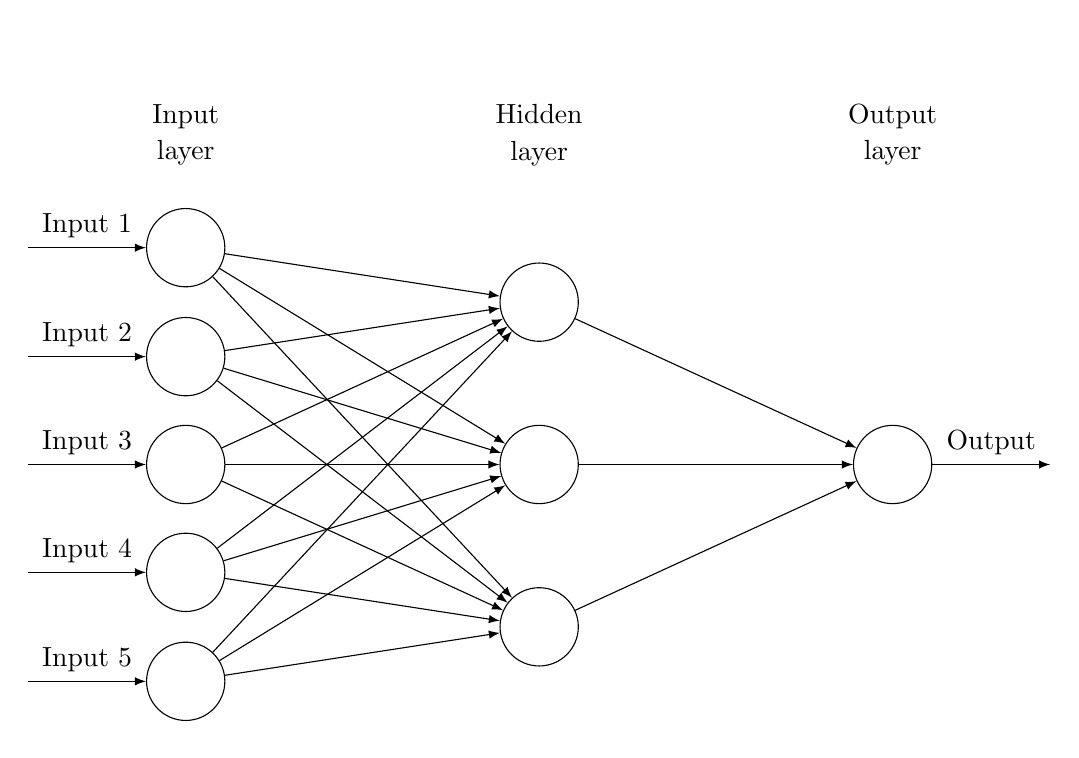
\begin{tikzpicture}[
    plain/.style={
      draw=none,
      fill=none,
    },
    net/.style={
      matrix of nodes,
      nodes={
        draw,
        circle,
        inner sep=10pt
      },
      nodes in empty cells,
      column sep=2cm,
      row sep=-9pt
    },
    >=latex
    ]
    \matrix[net] (mat)
    {
      |[plain]| \parbox{1.3cm}{\centering Input\\layer} & |[plain]| \parbox{1.3cm}{\centering Hidden\\layer} & |[plain]| \parbox{1.3cm}{\centering Output\\layer} \\
      & |[plain]| \\
      |[plain]| & \\
      & |[plain]| \\
      |[plain]| & |[plain]| \\
      & & \\
      |[plain]| & |[plain]| \\
      & |[plain]| \\
      |[plain]| & \\
      & |[plain]| \\    };
    \foreach \ai [count=\mi ]in {2,4,...,10}
    \draw[<-] (mat-\ai-1) -- node[above] {Input \mi} +(-2cm,0);
    \foreach \ai in {2,4,...,10}
    {\foreach \aii in {3,6,9}
      \draw[->] (mat-\ai-1) -- (mat-\aii-2);
    }
    \foreach \ai in {3,6,9}
    \draw[->] (mat-\ai-2) -- (mat-6-3);
    \draw[->] (mat-6-3) -- node[above] {Output} +(2cm,0);
  \end{tikzpicture}
  \centering
\end{figure}

\paragraph{} Given an input vector, a network can infer output values. This is computed by a forward pass which evaluates each neuron in turn, passing its value to the next layer along an edge. Each neuron performs the following calculation and returns $y$ with an input of vector $\textbf{x}$ in a forward pass.\cite{deeplearn}

\begin{align*}
  y &= \sigma(z) = \sigma \left(b + \sum_{i} x_{i} w_{i} \right)
\end{align*}

\paragraph{} The nonlinear function $\sigma$ enables the network to learn nonlinear functions. This project uses Rectified Linear Units (ReLU) and hyperbolic tangent activation functions for hidden and output layer neurons respectively. ReLU is the most popular activation function and is calculated by $\textrm{ReLU(}z) = \max(0, z)$, whereas $\tanh$ constrains the output to $(-1, 1)$. \cite{deeplearn}

\paragraph{} The weight vector $\textbf{w}$ and bias $b$ are parameters of each neuron. The set of all parameters of the network is referred to as the weights. These are updated in a backwards pass during training. A network with $n$ and $m$ neurons in the input and output layers respectively can be trained to approximate $\mathbb{R}^{n} \rightarrow \mathbb{R}^{m}$. A popular training algorithm is backpropagation. \cite{deeplearn}

\subsection{Backpropagation Learning Algorithm}

\paragraph{} Backpropagation utilises the multivariable chain rule to update the parameters of each neuron. It alters their parameters using first-order gradient descent calculated from a loss function measuring the difference between the observed and expected output values. A popular loss function is the Minimum Squared Error (MSE). \cite{deeplearn}

\begin{align*}
  C_{\text{MSE}} &= \frac{1}{2n} \sum_{i=0}^{n} \left(y_{observed, i}- y_{expected, i} \right)^{2}
\end{align*}

\paragraph{} Let $\delta^{l}_{i} = \frac{\partial C}{\partial z^{l}_{i}}$ is the change of cost with respect to neuron $i$ in layer $l$. Thus changes in output layer parameters are:

\begin{align*}
  \frac{\partial C}{\partial b^{l}_{i}} &= \alpha \delta^{l}_{i} \\
  \frac{\partial C}{\partial w^{l}_{i_{k}}} &= \alpha( y^{l-1}_{k} \delta^{l}_{i})
\end{align*}

\paragraph{} Here, the learning rate $\alpha$ amplifies and scales the change in weight for more efficient gradient descent. For weights in the output layer, $\delta^{output}_{i}$ for the $i^{\text{th}}$ can be calculated by

\begin{align*}
  \delta^{output}_{i} &= \frac{\partial C}{\partial y^{output}_{i}} \sigma ' (z^{output}_{i})
\end{align*}

\paragraph{} Otherwise,

\begin{align*}
  \delta^{l}_{i} &= \sum_{k} w^{l+1}_{k_{i}} \delta^{l+1}_{i} \sigma ' (z^{l}_{i})
\end{align*}

\paragraph{} Weight $w_{i_{k}}$, which connects neuron $i$ to $k$ can be updated thus, in a process known as stochastic gradient descent.

\begin{align*}
  w := w - \frac{\partial C}{\partial w^{l}_{i_{k}}}
\end{align*}

\paragraph{} Before training, the parameters of each neuron can be initialised to any starting value. To pick an unknown starting point, these values were randomised. Generally, larger networks need more data and thus training time to converge to a global minimum. Increasing the number of layers enable more complicated functions to be learnt, due to the composition of more simple functions. Increasing the number of neurons in hidden layers change local minima in gradient descent into saddle points. Training a network using (input, output) pairs is known as supervised learning.

\paragraph{} The architecture of the neurons, as well as the learning rate $\alpha$ are hyperparameters which are fixed before training. Hence training is often sensitive to hyperparameters. A method of finding a well-performing network architecture is cascade correlation.

\subsection{Finding Network Architecture using Cascade Correlation}

\paragraph{} Starting with a hidden layer of one neuron, cascade correlation finds the best architecture by incrementing neurons and layers, selecting the best performing architecture, as illustrated by Algorithm \ref{cascade}. The algorithm used in the project differs from the original in two ways. First, the best performing architecture is selected according to their accuracy on a testing set, instead of values of loss. Secondly, weights are randomised when new neurons are added, rather than keeping their values. This is because cascade correlation is used to find an architecture for reinforcement learning, trained with random weights. The original algorithm was intended to be applied to a dynamic supervised learning problem. \label{cascade}

\begin{algorithm}
  \caption{Cascade Correlation}
  Cascade correlation utilises the inputs $n_{input}, n_{output}, upper$. These represent the width of the input layer, output layer and the maximum width of a layer. The optimal performing architecture of hidden layers are stored in the parameter $hidden$.
  \begin{algorithmic}[1]
    \Function{cascadeCorrelation} {$n_{input}, n_{output}, upper$}
    \State $hidden \gets empty$
    \While {$hidden[\Call{length}{hidden}-1] > 1$}
    \State $bestScore = -1$
    \State $bestHidden$
    \For {each integer $i$ from 0 to $\Call{length}{hidden}$}
    \State $architecture \gets (n_{input}, hidden, i, n_{output})$
    \State $network \gets \Call{makeArchitecture}{architecture}$
    \State $\Call{train}{network}$
    \State $score \gets \Call{evaluate}{network}$
    \If {$score > bestScore$}
    \State $bestScore \gets score$
    \State $bestHidden \gets i$
	\EndIf
    \EndFor
    \State append $i$ to $hidden$
    \EndWhile
    \EndFunction
  \end{algorithmic}
\end{algorithm}

\section{Board Representation}

\paragraph{} As feedforward neural networks require one dimensional inputs, board representations convert two dimensional chessboards with twelve types of pieces into a representation vector. They are normalised to $(-1, 1)$ to increase the learning rate. Most chess engines have additional features in the representation vector which encode additional information, such as whether the King is in check or which pieces protect or attack others. These were not included in this project, because they can be expressed as linear functions of the pieces' coordinates. A good network architecture would be able to infer this information from the location of pieces. In addition, the inclusion of features may be partial to human bias. This is one of the first chess engines not to use additional information. The three main categories of board representations are presented below. \cite{giraffe} \cite{represent}

\subsection{Mailbox}

\paragraph{} The mailbox representation is a vector of length 64, each element corresponding to the squares on a chessboard. The value of each element is zero if no piece is present on the corresponding square. Otherwise, their value is given by the table below.

\begin{center}
  \begin{tabular}{ c | c  c }
    \hline
    \textbf{Piece} & \textbf{White} & \textbf{Black} \\ \hline
    Pawn & 1 & -1 \\
    Rook & 2 & -2 \\
    Knight & 3 & -3 \\
    Bishop & 4 & -4 \\
    Queen & 5 & -5 \\
    King & 6 & -6 \\
    \hline
  \end{tabular}
\end{center}

\subsection{Piece-List Coordinates}

\paragraph{} The piece-list representation is a flattened coordinate list of chesspieces. The order the coordinates appear in are given by the following table.

\begin{center}
  \begin{tabular}{c | c c c }
    \hline
    \textbf{Piece} & \textbf{Maximum Number of Pieces} & \textbf{White} & \textbf{Black} \\ \hline
    Pawn & 8 & 0 -- 7 & 8 -- 15 \\
    Rook & 10 & 16 -- 25 & 26 -- 35 \\
    Knight & 10 & 36 -- 45 & 46 -- 55 \\
    Bishop & 10 & 56 -- 65 & 66 -- 75 \\
    Queen & 9 & 76 -- 84 & 85 -- 93 \\
    King & 1 & 95 & 96 \\
    \hline
  \end{tabular}
\end{center}

\paragraph{} Rank and file coordinates of each piece are given below, with \{a -- h\} instead of \{1 -- 8\} for the file.

\begin{center}
  \medskip
  \newgame
  \showboard
\end{center}

\subsection{Bitboard}

\paragraph{} The bitboard board representation is similar to the mailbox board representation. Each piece can be represented as a tuple of (rank, file, piece type). This is used to index a third-order tensor of dimensions $\{8, 8, 12\}$. Elements in the tensor indexed by pieces are set to 1 and 0 otherwise. The resulting tensor is then flattened into a vector.

\begin{center}
  \begin{tabular}{c | c  c}
    \hline
    \textbf{Piece} & \textbf{White} & \textbf{Black} \\ \hline
    Pawn & 0 & 6 \\
    Rook & 1 & 7 \\
    Knight & 2 & 8 \\
    Bishop & 3 & 9 \\
    Queen & 4 & 10 \\
    King & 5 & 11 \\
    \hline
  \end{tabular}
\end{center}

\section{Reinforcement Learning}

\paragraph{} Reinforcement learning teaches an agent to play through experience. In this project, reinforcement learning trains a neural network to approximate an evaluation function by self-play. The resulting evaluation function is known as a value network. After a self-play game, a reward is returned to the agent. This is 1, 0 and -1 for a white win, draw and black win. These rewards are propagated to score every move in the game. Moves which occur closer to the end influence the reward more, whereas moves which occur earlier on may not impact the result as much. Thus rewards for moves which occur earlier should be discounted more. This process is done by temporal difference (TD) algorithms. TD learning algorithms used in this project are TD($\lambda$) \cite{TD-Gammon} and TD-Leaf($\lambda$) \cite{knightcap}.

\paragraph{} Training was done by self-play because of two reasons. First, an ideal opponent when training is one of similar strength. As the outcome would have an equal ratio of winning and losing, this prevents the agent to learn strategies for attack and defence simultaneously, avoiding bias towards one extreme. Secondly, self-play enables an engine to train without human intervention, which may be unknowingly flawed and suboptimal. \cite{ban}

\subsection{TD($\lambda$)}

\paragraph{} In a game of $T$ timesteps, let $\mathbf{x}_t$ be the board representation of the game at timestep $t$. Each $\mathbf{x}_t$ is associated with a value $v_t$ calculated from the evaluation function $f$ such that $f(\mathbf{x}_t) = v_t$. The reward returned by a move at timestep $t$ is thus the difference $d_{t}$ between two consecutive timesteps $v_{t+1} - v_{1}$.

\begin{align*}
  d_{T} &= reward - v_{T} \\
  d_{T-1} &= v_{T} - v_{T-1} \\
        &\mathrel{\makebox[\widthof{=}]{\vdots}} \\
  d_0 &= v_1 - v_0
\end{align*}

\paragraph{} If both players play optimally, both their value networks are optimal. In addition, if both follow a Minimax strategy, the players reach a Nash equilibrium, ensuring that neither player changes strategy. Therefore the value returned by the evaluation function would remain the same between timesteps: $v_{t} = v_{t+1}$. By transitivity, $v_0 = v_1 \ldots reward$. The value $v_{t}$ is said to back up $v_{t+1}$. Using the Minimum Squared Error, the cost function is

\begin{align*}
  \frac{1}{2} \sum_{i=0}^{T-1} \sum_{t=i}^{T-1} (v_{t+1} - f(\mathbf{x}_t))^2
\end{align*}

\paragraph{} During training, the value network will not be performing accurately, which may lead to the agent selecting suboptimal moves. Let the probability that $v_{t} = v_{t+1}$ is true be $\lambda$. This probability is known as the discount rate. Discounts follow a geometric progression such that a pair of values which are more timesteps apart are discounted more. With backups, the cost function is

\begin{align*}
  \frac{1}{2} \sum_{i=t}^{T-1} \sum_{t=i}^{T-1} \lambda^{i-t} (v_{t+1} - f(\mathbf{x}_t))^2
\end{align*}

\paragraph{} Gradient descent with the modified cost function yields the formula for updating weights according to TD($\lambda$).

\begin{align*}
  w &:= w - \nabla_w \frac{\alpha}{2} \sum_{i=t}^{T-1} \sum_{t=i}^{T-1} \lambda^{i-t} (v_{t+1} - f(\mathbf{x}_t))^2\\
  w &:= w + \alpha \sum_{i=t}^{T-1} \sum_{t=i}^{T-1} \lambda^{i-t} (v_{t+1} - f(\mathbf{x}_t)) \nabla_w f(\mathbf{x}_t)\\
  w &:= w + \alpha \sum_{i=t}^{T-1} \nabla_w f(\mathbf{x}_t) \sum_{t=i}^{T-1} \lambda^{i-t} (v_{t+1} - v_t))\\
  w &:= w + \alpha \sum_{i=t}^{T-1} \nabla_w f(\mathbf{x}_t) \sum_{t=i}^{T-1} \lambda^{i-t} d_t\\
  w &:= w + \alpha \sum_{i=t}^{T-1} \nabla_w f(\mathbf{x}_t) c_t
\end{align*}


where $c_t = \sum_{t=i}^{T-1} \lambda^{i-t} d_t$ is the eligibility trace. An easy way of computing it below.

\begin{align*}
  c_{t} &= \sum_{i=t}^{T-1} \lambda^{i-t} d_{i} \\
        &= d_{t} + \lambda c_{t+1}
\end{align*}

\paragraph{} At the edge cases $\lambda = 0$ and $\lambda = 1$, the following identities are noted.

\begin{align*}
  c_t &\equiv reward : \lambda = 0 \\
  c_t &\equiv v_{t+1} - v_t : \lambda = 1
\end{align*}

\paragraph{} When $\lambda = 0$, the equation becomes akin to Monte-Carlo methods, whereas $\lambda = 1$ methods are similar to dynamic programming methods. Hence intermediate values of $\lambda$ interpolate the two methods. A common value for $\lambda$ is 0.7. \cite{tdl}

\subsection{TD-Leaf($\lambda$)}

\paragraph{} Instead of backing up successive chessboard positions, TD-Leaf($\lambda$) backs up the leaf of the principle variation of each position. The principle variation is the best sequence of moves found by minimax. Its leaf node is the resultant board position after all principle variation moves.

\begin{center}
  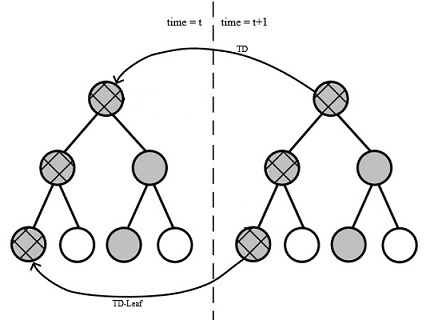
\includegraphics[scale=0.75]{td.png}
\end{center}

\paragraph{} The above picture adapted from \cite{meep} shows how values are backed up in TD($\lambda$) and TD-Leaf($\lambda$). Using the leaf instead of the search root speeds up learning. The update rule for TD-Leaf($\lambda$) is thus

\begin{align*}
  w &:= w + \alpha \sum_{i=t}^{T-1} \nabla_w f(pv(\mathbf{x}_t)) c_t
\end{align*}

\paragraph{} where $pv()$ is a function which returns the principle variation leaf of a board position.

\section{Requirements Analysis}

\paragraph{} After completing a literature review of chess engines and reinforcement learning, requirements to fulfil the project objective could be was defined, in order to refine a detailed implementation plan from the project proposal. Factors considered during the planning phase were programming languages, hardware, professional practice and ethical considerations.

\subsection{Deliverables}

\paragraph{} The initial plan was to adapt Giraffe to utilise \texttt{Python} neural networks. However, Giraffe's code is highly optimised and tightly integrated. An easier strategy was to adapt another chess engine such as Stockfish. There is a large research community using Stockfish, and its code is well commented and documented. Thus adapting Stockfish instead of Giraffe would increase accessibility of the project to a wider audience.

\paragraph{} A successful project would implement a trainable agent, a `random agent' playing randomly selected moves and a test suite to pit them against each other. As discussed above, the trainable agent requires search and evaluation functions as well as reinforcement learning algorithms. Performance of the value network could be improved by finding a good board representation and network architecture, as well as selecting good values for hyperparameters $\lambda$ and $\alpha$. The components, their priority and difficulty are summarised in the following table.

\begin{center}
  \begin{tabular}{l | l  l}
    \hline
    \textbf{Component} & \textbf{Priority} & \textbf{Difficulty} \\ \hline
    Search Algorithm & Medium & Medium \\
    Evaluation Function & High & Low \\
    Reinforcement Learning Algorithm & High & High \\
    Random Agent & High & Low \\
    Best Board Representation & Medium & Low \\
    Best Network Architecture & Medium & Medium \\
    Hyperparameter Optimisation & Low & Medium \\
    \hline
  \end{tabular}
\end{center}

%\paragraph{} Although the number of components is small, implementing each of the individual components efficiently and powerfully is challenging. In addition, the number of ways they could be combined is another challenge.

\subsection{Starting Point}

\paragraph{} The two languages used in the project are \texttt{C++} and \texttt{Python}. Most chess engines are written in \texttt{C++} due to speed and customisability. \texttt{Python} libraries such as \texttt{PyTorch} and \texttt{Keras} are currently the two most popular deep learning frameworks in research and industry. Both libraries were used to find the best. A table of software used and their starting point for learning is presented below.
% tensorflow backend

\begin{center}
  \begin{tabular}{l | l}
    \hline
    \textbf{Software} & \textbf{Starting Point} \\ \hline
    \texttt{Python} & Self-taught \\
    \texttt{PyTorch} & Online Tutorials \\
    \texttt{Keras} & Online Tutorials \\
    \texttt{C++} & Programming in \texttt{C/C++} (second year course) \\
    Giraffe & BitBucket Repository \\
    Stockfish & GitHub Repository \\
    Sunfish & GitHub Repository \\
    \hline
  \end{tabular}
\end{center}

\paragraph{} In addition, the courses Concurrent and Distributed Systems provided useful information in inter-process communications (IPCs) between \texttt{Python} and \texttt{C++}. Artificial Intelligence was useful for understanding neural networks. Knowledge of reinforcement learning was gained from reading Reinforcement Learning by Sutton and Barto as well as analysing the KnightCap, TD-Gammon and Giraffe.

\paragraph{} During implementation, a dataset of chess games was generated from data on the Free Internet Chess Server (FICS). This was used to compare board representations and network architectures.

\subsection{Ethical Considerations}

\paragraph{} A newly implemented chess engine could be a novel opponent humans could play against, recreationally or competitively. Chess engines are often used to analyse board positions and possible strategies. Any new knowledge the engine learnt would enable players to improve their understanding.

\paragraph{} The obvious commercial application of this project is a chess engine which plays against humans, providing feedback and guidance of possible moves. The engine could come untrained and gradually learn to predict and possibly counter the moves of a user, teaching both parties alike. Each chess engine would therefore be specifically tailored to its owner.

\paragraph{} Data taken from FICS was freely available. This was a database of internet chess games played in a public online forum since 2008. \cite{fics}

\section{Refined Plan}

\paragraph{} Due to the complexity in finding the best components for the project before their deployment in the final codebase, development was laid out in three stages.

\begin{enumerate}
\item Create baselines for machine learning and knowledge engineering chess agents, find the best libraries and packages.
\item Implement reinforcement learning algorithms, find best board representation, network architecture and hyperparameters.
\item Deploy neural network and search algorithm in a fast and efficient language such as \texttt{C++}, using a codebase such as Giraffe.
\end{enumerate}
  
\section{Software Engineering Practices}

\paragraph{} Software was developed according to the spiral model, with each stage a new spiral. Within each stage, Agile was used for rapid development. A kanban was used to visualise goals through the medium of a development flowchart. Prototypes were iteratively and modularly refined until the stage's goal was met.

\paragraph{} To prevent loss of data, code was backed up to \texttt{GitHub}, trained network weights were manually shared between computers and backed up to Google Drive. Each phase of the project was modular and kept in a distinct repository to prevent the git logs from being overwhelmingly long. New variants of algorithms were unit tested against previous versions.

\subsection{Hardware Used}

\paragraph{} Two machines were used in the project:

\paragraph{Macbook Pro, late 2015} (El Capitan, 16 GB RAM, 2.5 GHz Intel Core i7, 500 GB SSD) Used in code development and dissertation writing.

\paragraph{Desktop Computer} (Ubuntu, 32 GB RAM, 3.6 GHz Intel Core i7, Nvidia GeForce GTX 1080, 256 GB SSD) Used in code development, agent training, running and evaluation, due to its higher specs.

\paragraph{} If the above machines were to fail, an MCS machine, a research machine from the Computer Laboratory Computational Biology Group and the Cambridge High Performance Computing Services could replace the above devices through cloning the \texttt{GitHub} repositories and any required weights.

\section{Conclusion}

\paragraph{} Following a brief overview of algorithms and techniques used in the project, a refined plan was created to provide a structure for implementation. Details of how the value network, search algorithm and reinforcement learning algorithms were implemented are explained in the next chapter.


\chapter{Implementation}

\paragraph{} This chapter documents the implementation of the algorithms and plan discussed above. The three developmental phases of the spiral plan are chronologically documented, highlighting milestones in implementation. Challenges in developing and testing each component are elaborated with details of how they were resolved. The chapter concludes with a description of the final codebase. As evaluation of certain components of the chess engine influenced the development of the next stages during spiral development, some evaluations and analysis are presented along the way.

\section{Deep Learning with Giraffe}

%scope, performance; ease of implementation in various languages; isolate move generator
\paragraph{} In order to gauge the scope of the project, relevant libraries and programming languages were explored and analysed. To achieve this, Giraffe was adapted to utilise \texttt{Python} neural networks. The similarity between Giraffe and the architecture of this project's chess engine made it ideal for initial investigation. As it was developed in 2015, before deep learning libraries were developed, it utilised a neural network written in \texttt{C++} and ported to \texttt{Lua}. 

\paragraph{} Giraffe was well-documented with publicly available source code and weights. Its evaluation function is a 4 layer neural network. \cite{giraffe} This was reimplemented in \texttt{PyTorch} and \texttt{Keras}, to compare their performance with the original \texttt{C++} network. \texttt{Keras} is a library which is interpreted into \texttt{TensorFlow}, which itself calls \texttt{C++} subprocesses. \cite{tensorflow} \texttt{PyTorch} also wraps \texttt{C++}, but dynamically creates computational graphs and allocates resources. \cite{PyTorch} The weights were converted from a \texttt{t7} to \texttt{h5} format such that they could be imported in \texttt{PyTorch} and \texttt{Keras}. To interface these networks with \texttt{C++}, an IPC between the two languages was implemented such that Giraffe could evaluate chessboard positions using these \texttt{Python} networks. The resultant agent was pitted against \texttt{FairyMax} and the author within \texttt{XBoard} to determine their strength. \texttt{XBoard} was used to analyse the speed, search depth and moves considered by the agent. Speed of evaluation was found to be proportional to strength. \texttt{C++} was the fastest, followed by \texttt{PyTorch} and \texttt{Keras}. 

%\paragraph{} An unexaminable extension goal of the project was to create and train a chess engine with the AlphaGo architecture. The above experiment showed this goal to be infeasible, due to inadequate computational resources. AlphaGo utilises Monte-Carlo Tree Search (MCTS), which requires the result of hundreds of searches to be averaged. Within a 10 minute game, the result may not be reliable, due to a tradeoff between search depth and number of searches averaged. The average depth searched by Giraffe with a \texttt{Python} network was 8 plys, which is shallow compared to an average chess engine which can search up to 14 plys deep. However, the algorithm which trained AlphaGo was originally implemented in chess. Called TreeStrap, this algorithm can train alpha-beta search. Thus the extension goal was simplified to implementing and evaluating TreeStrap.

\paragraph{} After observing the performance of \texttt{Python} neural networks, the next step would be to implement TD($\lambda$) and TD-Leaf($\lambda$) in Giraffe. Their implementation required searching to return a list of nodes for temporal difference backups. Thus the search algorithm would have to be reimplemented, requiring the move generator to be isolated. To gain a deeper understanding of the source code, UML diagrams were generated using BoUML. These diagrams revealed a highly optimised and occasionally underdocumented class hierarchy. Modifying other chess engines for reinforcement learning was easier, even though \texttt{Python} neural networks had already been successfully incorporated in Giraffe. The alternative would be to implement the search algorithm and move generator from scratch. As many efficient implementations already exist in numerous chess engines, this would be an inefficient use of time to obtain a suboptimal result.

\section{Rapid Prototyping in  \texttt{Python}}

% toy problem
\paragraph{} Having observed the performance of an evaluation function using trained weights from Giraffe, strategies for training it needed to be found. Factors which could affect training rate were the network architecture, board representation and training hyperparameters. The best configuration of all components needed to be determined for efficient training. In addition, reinforcement learning algorithms for training needed to be implemented and verified. As the Giraffe move generator was not going to be used, an alternative was found in Sunfish. This chess engine is written in 111 lines of \texttt{Python}, enabling the whole engine to be analysed and the move generator quickly identified. \cite{sunfish} \texttt{Python} was chosen as the language for rapid prototyping, testing and evaluation because it is terse, interpretive, and high-level. In contrast, the final codebase would be developed in \texttt{C++} for speed and efficiency.

%\paragraph{} Performance of deep reinforcement learning depends on the network architecture, which itself depends on which board representation is used. The logical order for developing these components would be to start from board representation and end with reinforcement learning.

\subsection{Analysing Representations with Supervised Learning}

% find best
\paragraph{} The most obvious strategy to analyse board representation and network architecture would be to implement the whole reinforcement learning algorithm and observe how changing their configuration affects training. This is inefficient because reinforcement learning does not intensively train the network. More time is spent searching and generating moves instead. A more network-intensive training strategy is supervised learning.

\paragraph{} Section 2.3 shows that the evaluation function approximates $\mathbb{E} \giventhat{reward}{representation}$. Another way this can be approximated is to train a network to predict the winner given a chessboard representation. Values for black and white checkmate were set to $-1, 1$, making this a supervised classification problem. An alternate approach was supervised regression against normalised values of Stockfish's evaluation function. The shortcomings of this approach were in difficulty of testing and dissimilarity of datasets. Stockfish's evaluation function ranks the favourability of the next move rather than predicting the eventual winner. \cite{stockfish} Training the network to predict normalised values would be a different function than predicting the winner from a chessboard position. Supervised classification is a better approach because accuracy of predictions could be easily calculated using a validation set.

% generate data
\paragraph{} Training data was generated from the Free Internet Chess Server (FICS) database, a record of all games played on the eponymous server since 2008. \cite{fics} These games can be viewed by the public in real time. Games from 2017 and 2016 were used to generate the supervised learning dataset. The downloaded dataset was in \texttt{.pgn} format, consisting of a list of games. Each game recorded the moves played, the online handles of the players, their strengths and the outcome. Only games which ended in checkmate were utilised for training. Games which ended in resignations, draws and stalemates were ignored, in order to simplify the dataset as much as possible. In addition, only games where both players were over 1500 ELO were used. ELO scores the strength of a player, and is around the level of a seasoned amateur. Filtering out games played by weaker players reduced the probability of a player winning through their opponent's blunder, reducing noise in the dataset. Hence a more favourable board positions for a player would more likely lead to their checkmate.

\paragraph{} A training and testing set of 500000 and 50000 datapoints was generated, because 500000 is roughly the square of the number of neurons in the largest network. These sets were partitioned such that a datapoint used in training would not reappear in testing. Testing data would be drawn from the same distribution of datapoints but would not have been previously seen.

\paragraph{} The chessboard position was represented in Forsyth-Edwards Notation (FEN) string, a representation described fully in Appendix A. Chessboard positions were selected at a random point in the game. The parameter $gamestage$ was a fraction representing how far the game has progressed. A value of 0.5 meant that the game was halfway, and a value of 1.0 meant that the game was over. This parameter served as a lower bound from which a position could be drawn, with 1.0 as the upper bound. After converting this position to a FEN, datapoints of (FEN, winner) tuples could be saved as a \texttt{.csv}. The following algorithm shows how this file was generated in pseudocode.

\begin{algorithm}
  \caption{Generated Supervised Classification Dataset from FICS}
  The function $\Call{generateFEN}{}$ writes a list of FENs representing board position and the eventual winner from this position in $outFile$. The FENs are generated from $FICSfile$ and is the size of $sizeOfDataset$. The parameter $gameStage$ is a float in the range $(0.0, 1)$.
  \begin{algorithmic}[1]
    \Function{generateFEN} {$FICSFile, gameStage, sizeOfDataset, outFile$}
    \While {integer $games < sizeOfDataset$}
    \State $game \gets FICSFile.nextGame$
    \If {$game.playerStrength > 1500$ \textbf{and} $game.checkmate$}
    \State $games \gets games + 1$
    \State $board \gets startingPosition$
    \State $ply \gets integer(\Call{randomFloat}{gameStage, 1.0} * game.length)$
    \While {integer $count < ply$, increment count}
    \State $\Call{move}{board, game.getNextMove}$
    \EndWhile
    \State $\Call{writeAsFEN}{outFile, board, game.winner}$
    \EndIf
    \EndWhile
    \EndFunction
  \end{algorithmic}
\end{algorithm}

\paragraph{} The algorithm was implemented in \texttt{Python}, utilising the \texttt{Python-Chess} library. This library was used to read the FICS \texttt{.pgn} file and convert a FEN string to and from its own board representation, that of a mailbox (Section 2.4.1). Functions converting the \texttt{Python-Chess} mailbox to seven other board representations were created, such that a FEN could be converted into one of the seven representations to be analysed. In addition to the three board representations described in Section 2.4, one other variant of bitboard and three variants of piece-list coordinates were used.

\paragraph{} The alternative bitboard representation reduces its dimensions to $\{8, 8, 6\}$. Elements in the tensor are initialised to 0. A white piece would set its index ($rank$, $file$, $pieceType$) to 1, and -1 if the piece is black. After flattening, this representation was known as an antisymmetric bitboard.

\paragraph{} Many of the values within a piece-list coordinate representation are 0 because it was unlikely that pawns were ever going to be promoted to fill them. Creating a piece-list according to the following table would statistically reduce the representation size without losing information. Board representations generated using the following table are called compressed piece-lists.

\begin{center}
  \begin{tabular}{c | c c c}
    \hline
    \textbf{Piece} & \textbf{Number of Pieces} & \textbf{White} & \textbf{Black} \\ \hline
    Pawn & 8 & 0 -- 7 & 8 -- 11 \\
    Rook & 4 & 12 -- 15 & 16 -- 19 \\
    Knight & 4 & 20 -- 23 & 24 -- 31 \\
    Bishop & 4 & 32 -- 35 & 36 -- 39 \\
    Queen & 4 & 40 -- 43 & 44 -- 48 \\
    King & 1 & 49 & 50 \\
    \hline
  \end{tabular}
\end{center}

\paragraph{} Two coordinate representations for piece-lists were used, one with a simple $(rank, file)$ and the other with $(rank, 9-rank, file, 9-file)$. The second representation ensures that the magnitude of a piece's coordinates do not vary with its location of pieces. Representations which have two coordinates per piece are known as small piece-lists.

% variety of networks
\paragraph{} These seven representations were analysed with different network architectures and $gameStage$ values. Values of $gameStage$ were 0.5 and 0.75, and three architectures were used. These architectures were:

\begin{enumerate}
\item \textbf{Small Network}: Single neuron with tanh activation function. Many chess engines use this because of efficiency. If used without an activation function, the computation is a linear combination.
\item \textbf{Medium Network}: Has a hidden layer of 64 neurons.
\item \textbf{Large Network}: Giraffe Neural Network with two hidden layers, adapted for different board representations. The first hidden layer has an equal number of neurons as the input layer and the second hidden layer has 64 neurons.
\end{enumerate}

\paragraph{} For reliability, the networks were trained ten times, each time starting from a different random parameter instantiation. After testing, the means and standard deviations of the accuracies were computed. Unfortunately, the differences between each network were negligible and statistically insignificant, less so for $gameStage = 0.75$. To obtain as significant a difference as possible, the networks were trained again with a dataset where $gameStage = 1.0$. This dataset only contained checkmate positions. The results after training on this dataset is shown in the graph below, alongside very small standard deviation error bars.

\begin{center}
  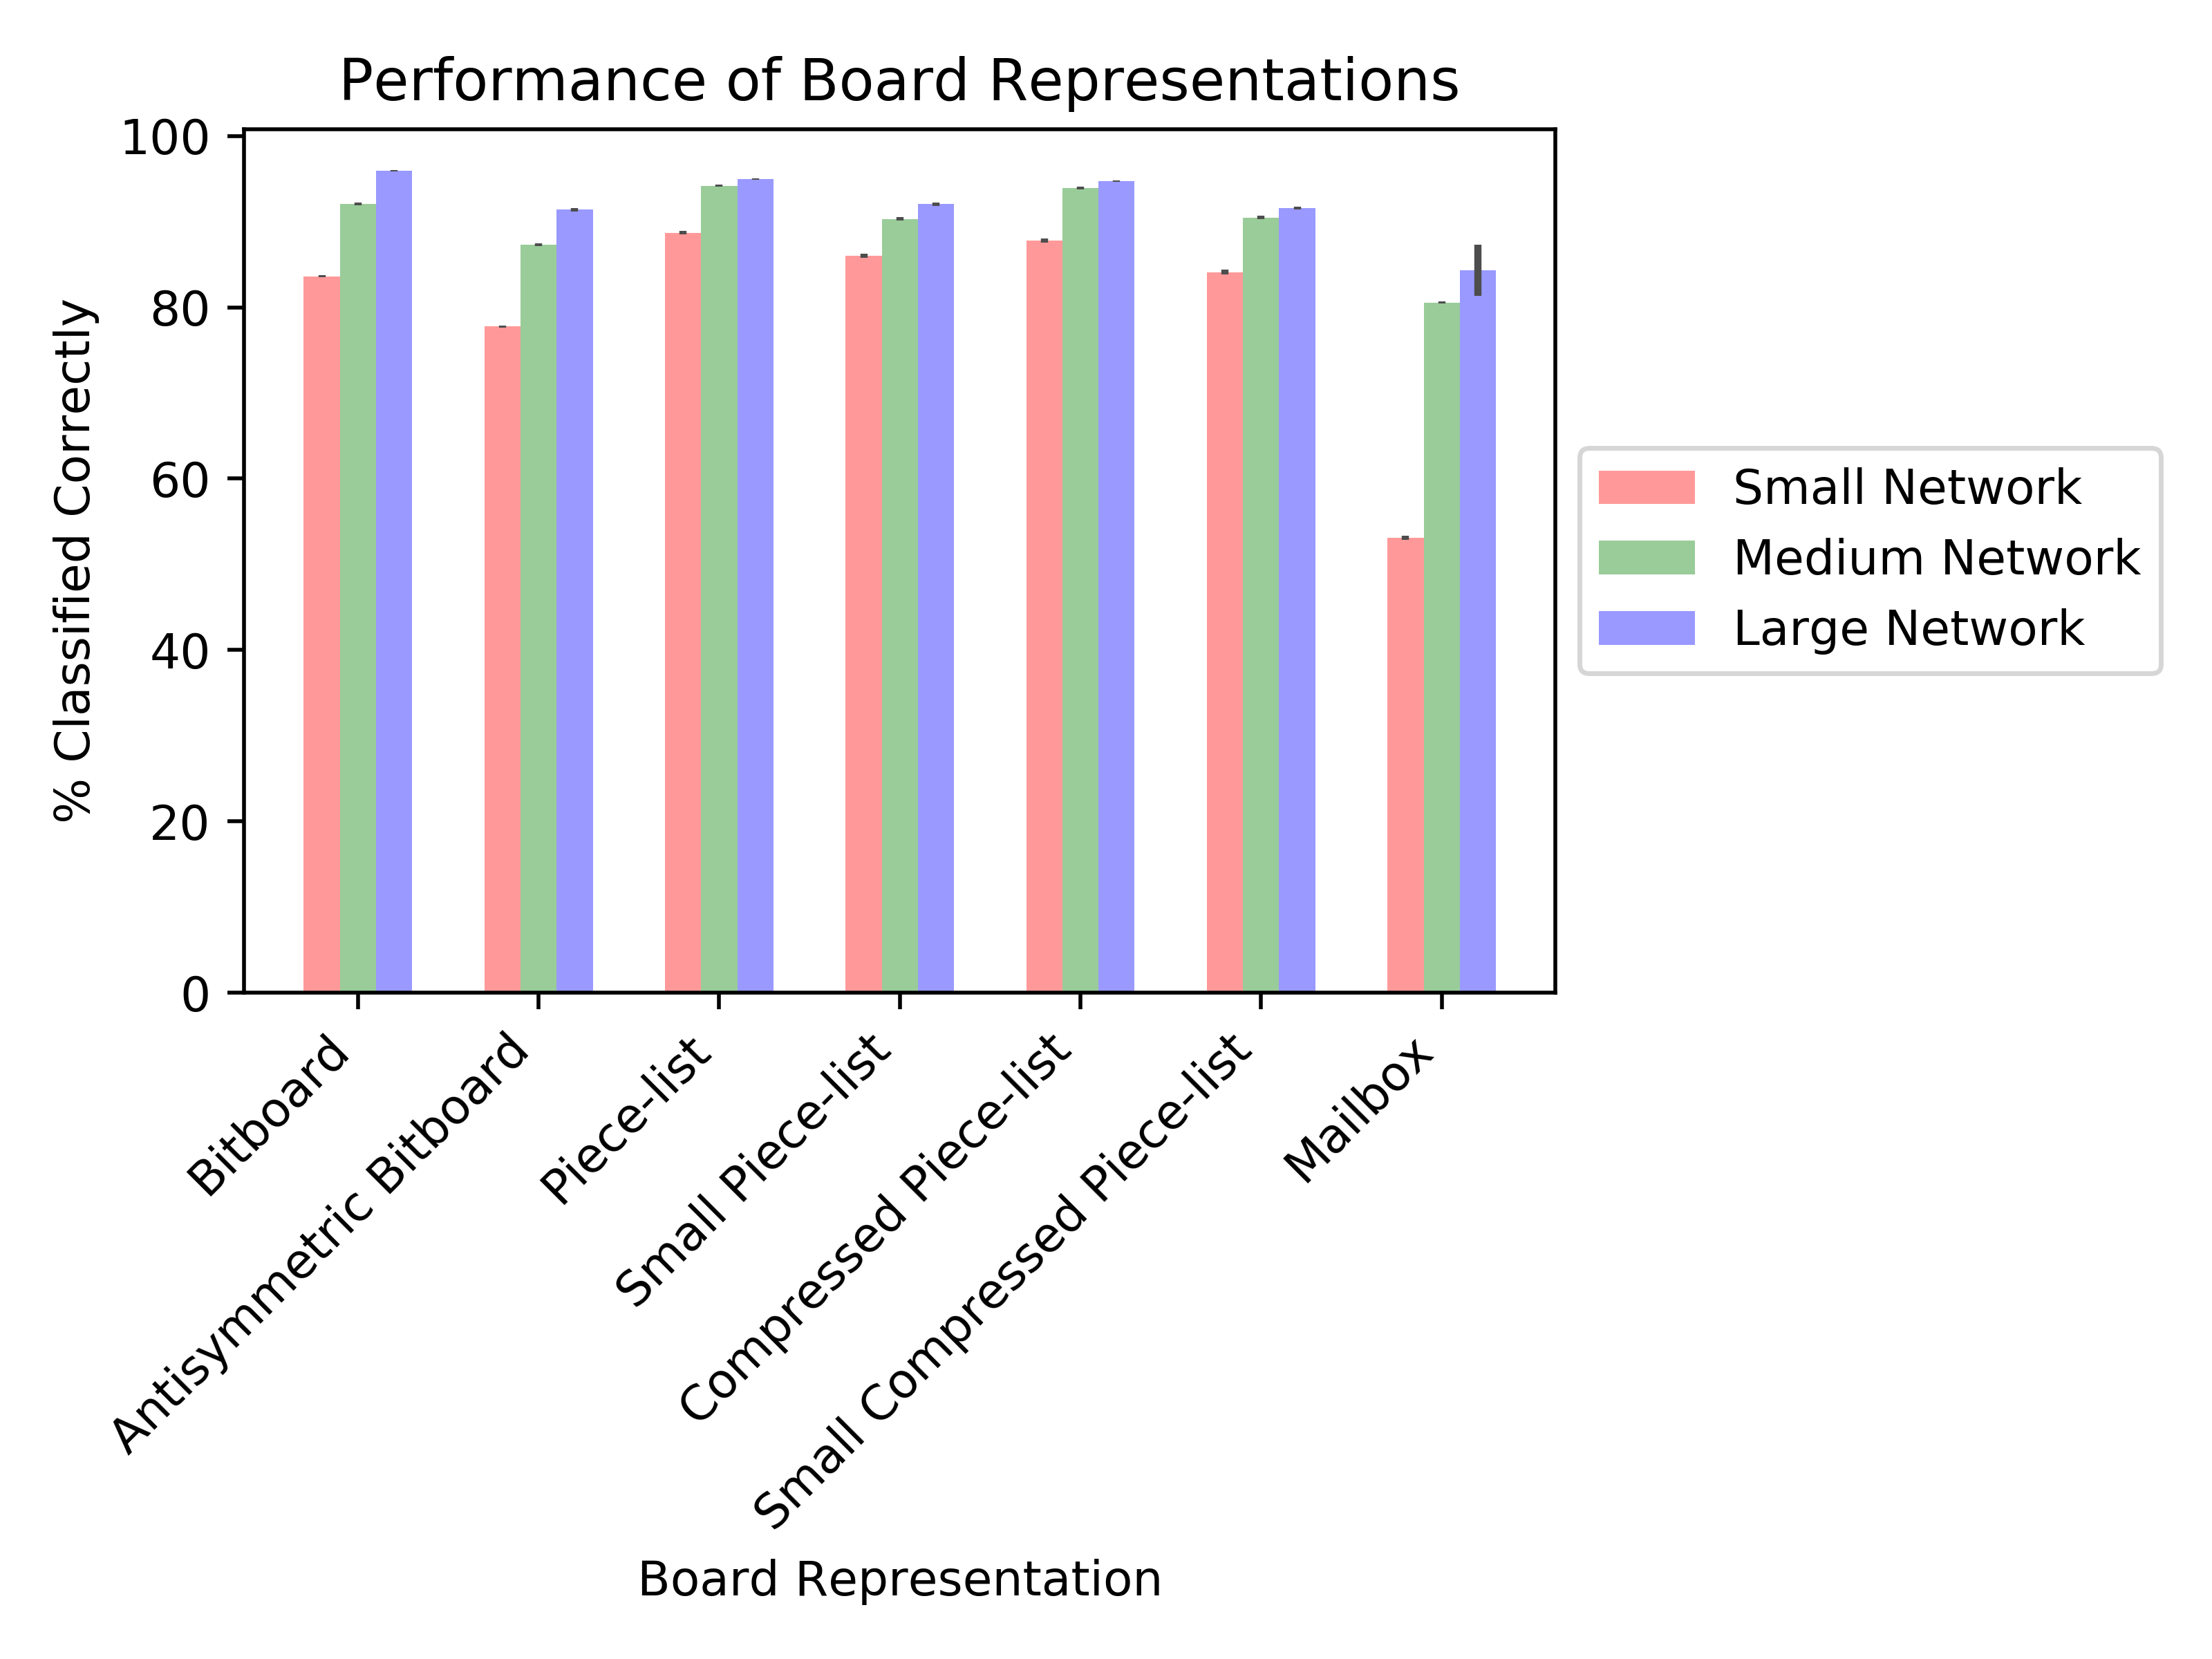
\includegraphics[scale=0.9]{boardrepr.png}
\end{center}
  
\paragraph{} This graph showed significant differences between the accuracies. Overall, the piece-list representation produced the best results. Using this representation, cascade correlation was then used to find a good architecture. It was surprising to observe that the compressed piece-list produced a very similar result, as hypothesised.

\subsection{Finding Network Architectures with Cascade Correlation}

\paragraph{} Having concluded that the piece-list representation produced the best results, this was used as the input layer of a neural network. To find the architecture of the hidden layers, cascade correlation was used to find network architectures. The algorithm was implemented using \texttt{Python}, \texttt{PyTorch} and \texttt{Python-Chess} and trained on the checkmate dataset.

\paragraph{} A final architecture returned was \{384, 315, 80, 10, 5, 2, 1\}. However, this algorithm was not numerically stable given different random initialisations of network weights. Due to the lack of consistent results, and the good scores of networks used in the previous section, the Small and Medium Networks were used as network architectures in subsequent sections. As results between the Large and Medium Networks were similar, the Large Network was not used due to substantially longer training time.

\subsection{Implementing TD($\lambda$) with Sunfish}

\paragraph{} Now that a network architecture has been found, deep reinforcement learning algorithms could be developed and verified quickly. This required creating a custom loss function and weight updater. In order to create these functions, an existing implementation of Negamax was modified to return a list of boards and values such that temporal difference values could be calculated. In addition, the neural network was used in evaluation. Overall, extracting the move generator from Sunfish was a lot more straightforward compared to Giraffe.

% isolate move generator
\paragraph{} The move generator returned all possible moves, including illegal moves such as placing the King into check or, through inaction, allowing it to be captured. Such illegal moves had to be filtered out. In addition, Sunfish could not recognise draws, checkmates or stalemates. A function which recognised these different states was created such that rewards could be assigned to players at the conclusion of a game. 

% TD-Lambda
\paragraph{} The loss function and weight update for TD($\lambda$) was implemented in \texttt{Python} using \texttt{PyTorch} primitives. This enabled temporal difference arithmetic to be calculated using the GPU, in addition to backpropagation algorithm. As neither TD($\lambda$) or TD-Leaf($\lambda$) is commonly used, they were not part of the \texttt{PyTorch} repository, and had to be custom developed from scratch. The temporal difference equation and weight updater are

\begin{align*}
  \frac{1}{2} \sum_{i=t}^{T-1} \sum_{t=i}^{T-1} \lambda^{i-t} (v_{t+1} - f(\mathbf{x}_t))^2
\end{align*}
\paragraph{} and
\begin{align*}
  w &:= w + \alpha \sum_{i=t}^{T-1} \nabla_w f(\mathbf{x}_t) c_t
\end{align*}

\paragraph{} \texttt{PyTorch} numerically computes gradients by the AutoGrad method, amortising the computation of calculating derivatives. These derivatives can be numerically computer after a forward pass, meaning that the derivatives for each parameter has already been computed. This simplifies the process to write custom loss and gradient descent weight updaters, as backpropagation does not need to be reimplemented. The combined function for temporal difference learning is presented below.

\begin{verbatim}
  def temporal_difference(self, boards, result):
        'temporal difference learning with boards and results'
        # boards is a list of chessboard positions in the game,
        # going chronologically forwards
        v = torch.cat([result] + [self(Variable(x)) for x in boards[::-1]])
        d = (v[:-1] - v[1:]).detach()
        v = v[:-1]
        
        # loss is calculated according to the temporal-difference equation
        trace = Variable(torch.cuda.FloatTensor(len(boards)).fill_(0.0))
        trace[0] = trace[0] + d[0]
        for t in range(1, len(boards)):
            trace[t] = trace[t] + d[t] + self.DISCOUNT_RATE * trace[t-1]
        epsilon = -(v * trace).sum()
        epsilon.backward()
        print "change of weights epsilon", epsilon.data[0]
        
        # p.grad.data is a numerically computed derivative
        for p in self.parameters():
            p.data -= self.LEARNING_RATE * p.grad.data
            
        # zero all the numerically computed derivatives
        for p in self.parameters():
            p.grad.data.zero_()
\end{verbatim}

\paragraph{} If \texttt{boards} was a list of leaf nodes of searches, the above function would update the weights of a network according to TD-Leaf($\lambda$)

\paragraph{} TD($\lambda$) was also implemented for the \texttt{Keras} neural network. The \texttt{PyTorch} version was superior because of its speed, efficient allocation of GPU and CPU memory and lack of memory leaks. The memory leak in \texttt{Keras} had been thoroughly documented at the time of development with no solution. Numerical differentiation used in \texttt{PyTorch} utilises dynamic memory management. \texttt{Keras} is a wrapper for \texttt{TensorFlow}, which allocates memory statically, before the derivatives are calculated. As deep reinforcement learning is an online learning method, calls to run and train are dovetailed, and training depends on what values have just been run. Hence \texttt{TensorFlow} was creating a new static graph every time a game was played. Memory used for this graph was not freed after the derivatives were computed and the weights updated, thus consuming increasing memory. Resolving this issue is difficult in \texttt{Python} because there are no memory management operators. This complicated by the fact that \texttt{Keras} is a wrapper of \texttt{TensorFlow}, which calls the \texttt{C++} functions to allocate and deallocate memory. \cite{tensorflow} After considering all the above, neural networks in the project would be written in \texttt{PyTorch}.

\subsection{Implementing a Random Agent}

\paragraph{} The random agent is an adversary which plays randomly selected moves. Pseudocode of the agent is given below.

\begin{algorithm}
  \caption{Random Agent}
  The function $\Call{moveRandom}{}$ returns a randomly generated move from chessboard position $position$.
  \begin{algorithmic}[1]
    \Function{moveRandom} {$position$}
    \If {$\Call{noFurtherPossibleMoves}$}
    \State \textbf{return} $\_$
    \EndIf
    \State $max \gets -\infty$
    \State $maxMove$
    \For {$move$ in \Call{moveGenerator}{$position$}}
    \State $score \gets \Call{random}{}$
    \If {$score \geqslant max$}
    \State $max \gets score$
    \State $maxMove \gets move$
	\EndIf
    \EndFor
    \State \textbf{return} $maxMove$
    \EndFunction
  \end{algorithmic}
\end{algorithm}

\subsection{Convergence of Learning Algorithms Using an Endgame}

\paragraph{} To verify that the learning algorithms had been implemented correctly, agents were trained in a subproblem of chess known as an endgame. As its name suggests, an endgame occurs towards the end of a chess game, where only a few pieces remain. Checkmate for one player is usually a foregone conclusion depending on which pieces are present. The few pieces reduces the branching factor and the problem size, thus enabling learning to converge faster. This project used the king rook and king (KRvK) endgame because it was small enough such that a unique dominant strategy for checkmate exists. In contrast, a king, queen and king (KQvK) endgame has many strategies for checkmate. It is easier for the checkmate to occur by chance in KQvK, making it harder to distinguish between whether the agent has learnt a good strategy or has blundered into checkmate.

\paragraph{} The starting point for the KRvK endgame is shown below, with White to move.

\begin{center}
  \medskip
  \fenboard{1k6/8/2K5/3R4/8/8/8/8 w - - 0 0}
  \showboard
\end{center}

\paragraph{} The three move dominant strategy yielding checkmate is described below. As this is the only way to generate checkmate in three moves, the optimality of an agent's behaviour can be determined by human inspection.

\begin{center}
  \begin{tabulary}{\linewidth}{LLL}
    \medskip
    \fenboard{1k6/8/2K5/R7/8/8/8/8 w - - 0 0}
    \scalebox{0.75}{\showboard}
    \medskip
    &
    \medskip
    \fenboard{2k5/8/2K5/R7/8/8/8/8 w - - 0 0}
    \scalebox{0.75}{\showboard}
    &
    \medskip
    \fenboard{R1k5/8/2K5/8/8/8/8/8 w - - 0 0}
    \scalebox{0.75}{\showboard}
    \\
    White moves their castle from $d5$ to $e5$ \ldots
    &
    forcing black to move from $b8$ to $c8$ \ldots
    &
    white moves $e5$ to $a8$: Checkmate!
    \\
  \end{tabulary}
\end{center}

\paragraph{} In addition, training speed was increased by using the small network architecture. The following graphs confirms that the algorithm has been implemented correctly. The upper subplot then reveals that the strategy which is being converged upon yields a checkmate in three moves -- the strategy described above. The grey dots representing loss tends towards zero with the number of games increasing, implying that the strategy learnt by the agent is converging. The cumulative number of wins and draws show a mixture of both results at first, before the agent learns to win every time.

\begin{absolutelynopagebreak}
\begin{center}
  \centerline{Training an Agent on a KRvK Endgame using TD($\lambda$)}
  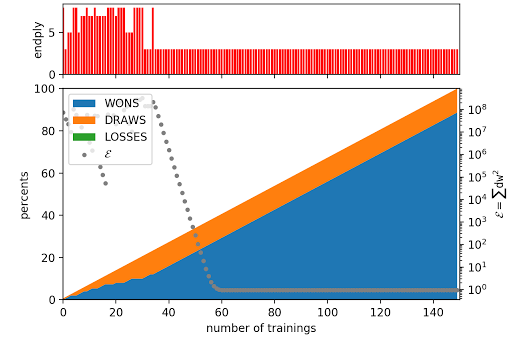
\includegraphics[scale=0.7]{tdlambdaloss.png}
\end{center}
\end{absolutelynopagebreak}

% TD Leaf
\paragraph{} TD-Leaf($\lambda$) was trained on the same subproblem as TD($\lambda$). The results were similar, with TD-Leaf($\lambda$) converging faster than TD($\lambda$). Values for hyperparameters were found using trial and error. $\alpha$ and $\lambda$ were set to 0.01 and 0.7.

\begin{absolutelynopagebreak}
\begin{center}
  \centerline{Training an Agent on a KRvK Endgame using TD-Leaf($\lambda$)}
  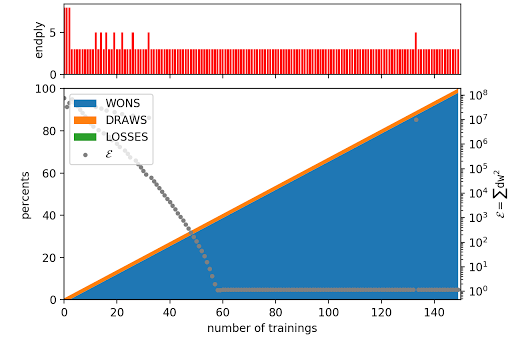
\includegraphics[scale=0.7]{tdleafloss.png}
\end{center}
\end{absolutelynopagebreak}

\paragraph{} Loss gradually converged in TD-Leaf($\lambda$), rather than fluctuating a lot in TD($\lambda$). This implies that TD-Leaf($\lambda$) is a stronger training algorithm capable of producing better results. This is confirmed by the ratio of draws : wins being much lower in TD-Leaf($\lambda$). An agent trained with TD-Leaf($\lambda$) would be capable of learning better strategies in fewer time.

\paragraph{} The loss in training converged after 60 training games for both algorithms because the same architecture and hyperparameters were used. Hence their convergence rates are expected to be at the same rate.

\subsection{Preparing for Deployment}

% more features, less error-prone, faster
\paragraph{} Since all the components had been implemented and had been used to solve a toy subproblem, the next step would be to deploy and train the algorithm on the entire game of chess. However, there were some limitations to the Sunfish engine. There was a lack of underpromotion and en passant, and the move generator was error-prone. Hence the Sunfish move generator was replaced with one from the \texttt{Python-Chess} library. Although not intended to deploy competitive chess engines, the \texttt{Python-Chess} was straightforward to use and faster than Sunfish.

\paragraph{} An obvious problem with this engine is its speed of searching. Within a ten minute game, an agent could only search to 2 plys depth, a lot slower than the average value of 14 for many chess engines. This problem would be solved by deploying in \texttt{C++} in the next stage. Despite the slow speed, agent behaviour shared some similarity with other reinforcement learning projects.

% exploration and exploitation 
\paragraph{} The agent would often play the same sometimes suboptimal game again and again, instead of finding a better strategy. This is because the agent is not currently exploring the environment and is exploiting the same strategy. Balancing exploration and exploitation is a fundamental tradeoff in reinforcement learning. After the agent has explored the environment sufficiently, it can then learn and exploit the best strategy.

\paragraph{} To increase exploration, draws by repeated moves or 50-plys were ignored in favour of playing towards checkmate or stalemate, such that board positions which would hitherto be unseen could be explored. In addition, the first four moves of each game would be randomly selected, ensuring that there would be a variety of games played.

\section{Deployment in Stockfish and \texttt{C++}}

\paragraph{} Stockfish is one of the most powerful chess agents in the world, used and maintained by an active community. The source code is open-source and liberally commented, making Stockfish easy to adapt and this project accessible to a wide audience. The final codebase would modify Stockfish to train and use a neural network as an evaluation function.

% deployment oriented, why stockfish
\paragraph{} In the previous phase, TD($\lambda$) and TD-Leaf($\lambda$) were implemented and verified. In addition, good board representations and network architectures were found and implemented. In order to utilise these features in as strong a chess agent as possible, the fastest possible configurations of searching algorithm, neural network library and move generator should be found.

% C++ > PyTorch > Tensorflow
\paragraph{} Weights trained with \texttt{PyTorch} could be exported and run in \texttt{Caffe2}, a deployment-oriented submodule of \texttt{PyTorch}. Both libraries could be run with or without GPU acceleration. The time to evaluate 10000 board positions was calculated, producing the following graph. Ten repeated readings were generated with varying load, enabling a standard deviation to be found and plotted as error bars. Variable load was achieved by running a different number of invocations of the program in parallel.

\begin{center}
  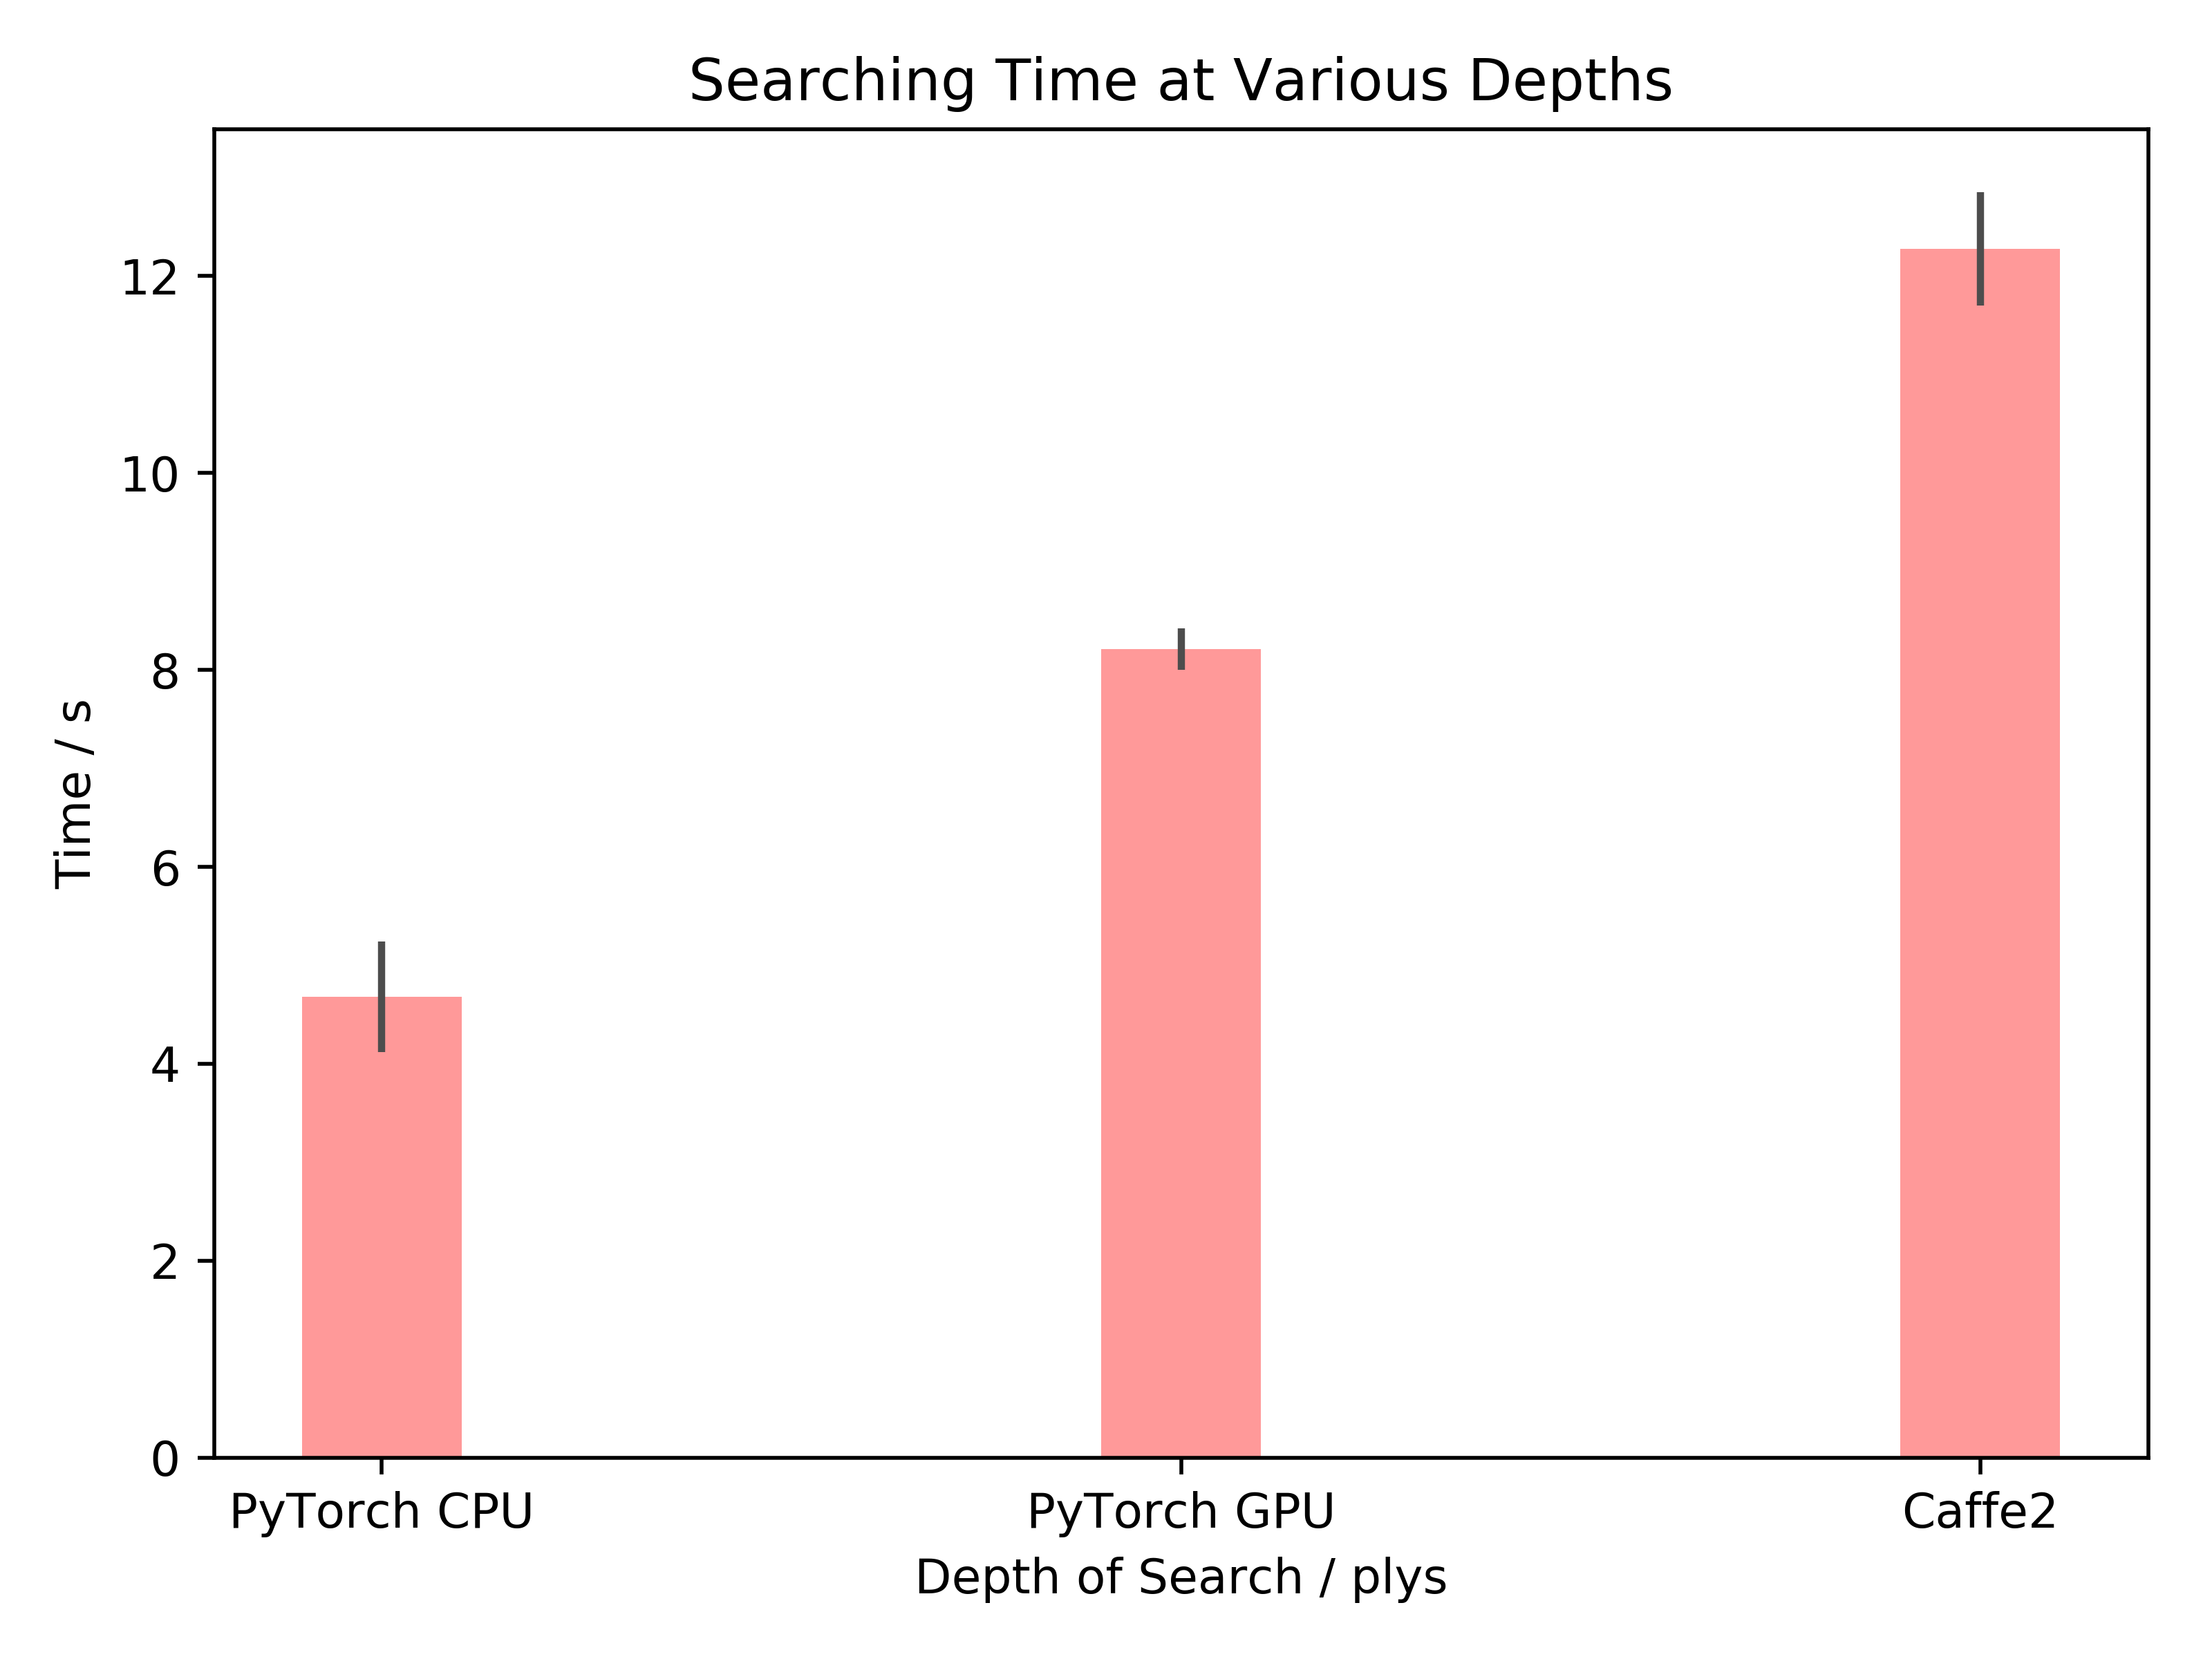
\includegraphics[scale=0.8]{ipc.png}
\end{center}

\paragraph{} As the neural networks used are relatively small compared to state-of-the-art deep networks, the GPU is underutilised and is slower than running on just the CPU. Copying arrays to and from the GPU added an overhead to which slowed down inference. If the network was larger, this overhead would have been negligible compared to the speedup the GPU could provide due to computing many arithmetic operations in parallel.

\paragraph{} The \texttt{Caffe2} framework has a structure similar to that of \texttt{TensorFlow}, as graphs were also statically allocated. This similarity could be the reason why \texttt{Caffe2}, like \texttt{TensorFlow} is slower than \texttt{PyTorch}.

\paragraph{} An even faster implementation of neural networks would be to implement the neural networks from scratch in \texttt{C++}, as Giraffe does. This possible future research direction is left open to the interested reader. 

\paragraph{} To compare the speed of Stockfish's move generator with Sunfish and \texttt{Python-Chess}, searches of depth 0 -- 5 were timed for Negamax with no pruning, producing the following graph with a logarithmic y-axis. Reliability was ensured by repeating the timings ten times, again with varying CPU load. This enabled standard deviation error bars to be plotted on the following graph.

\begin{center}
  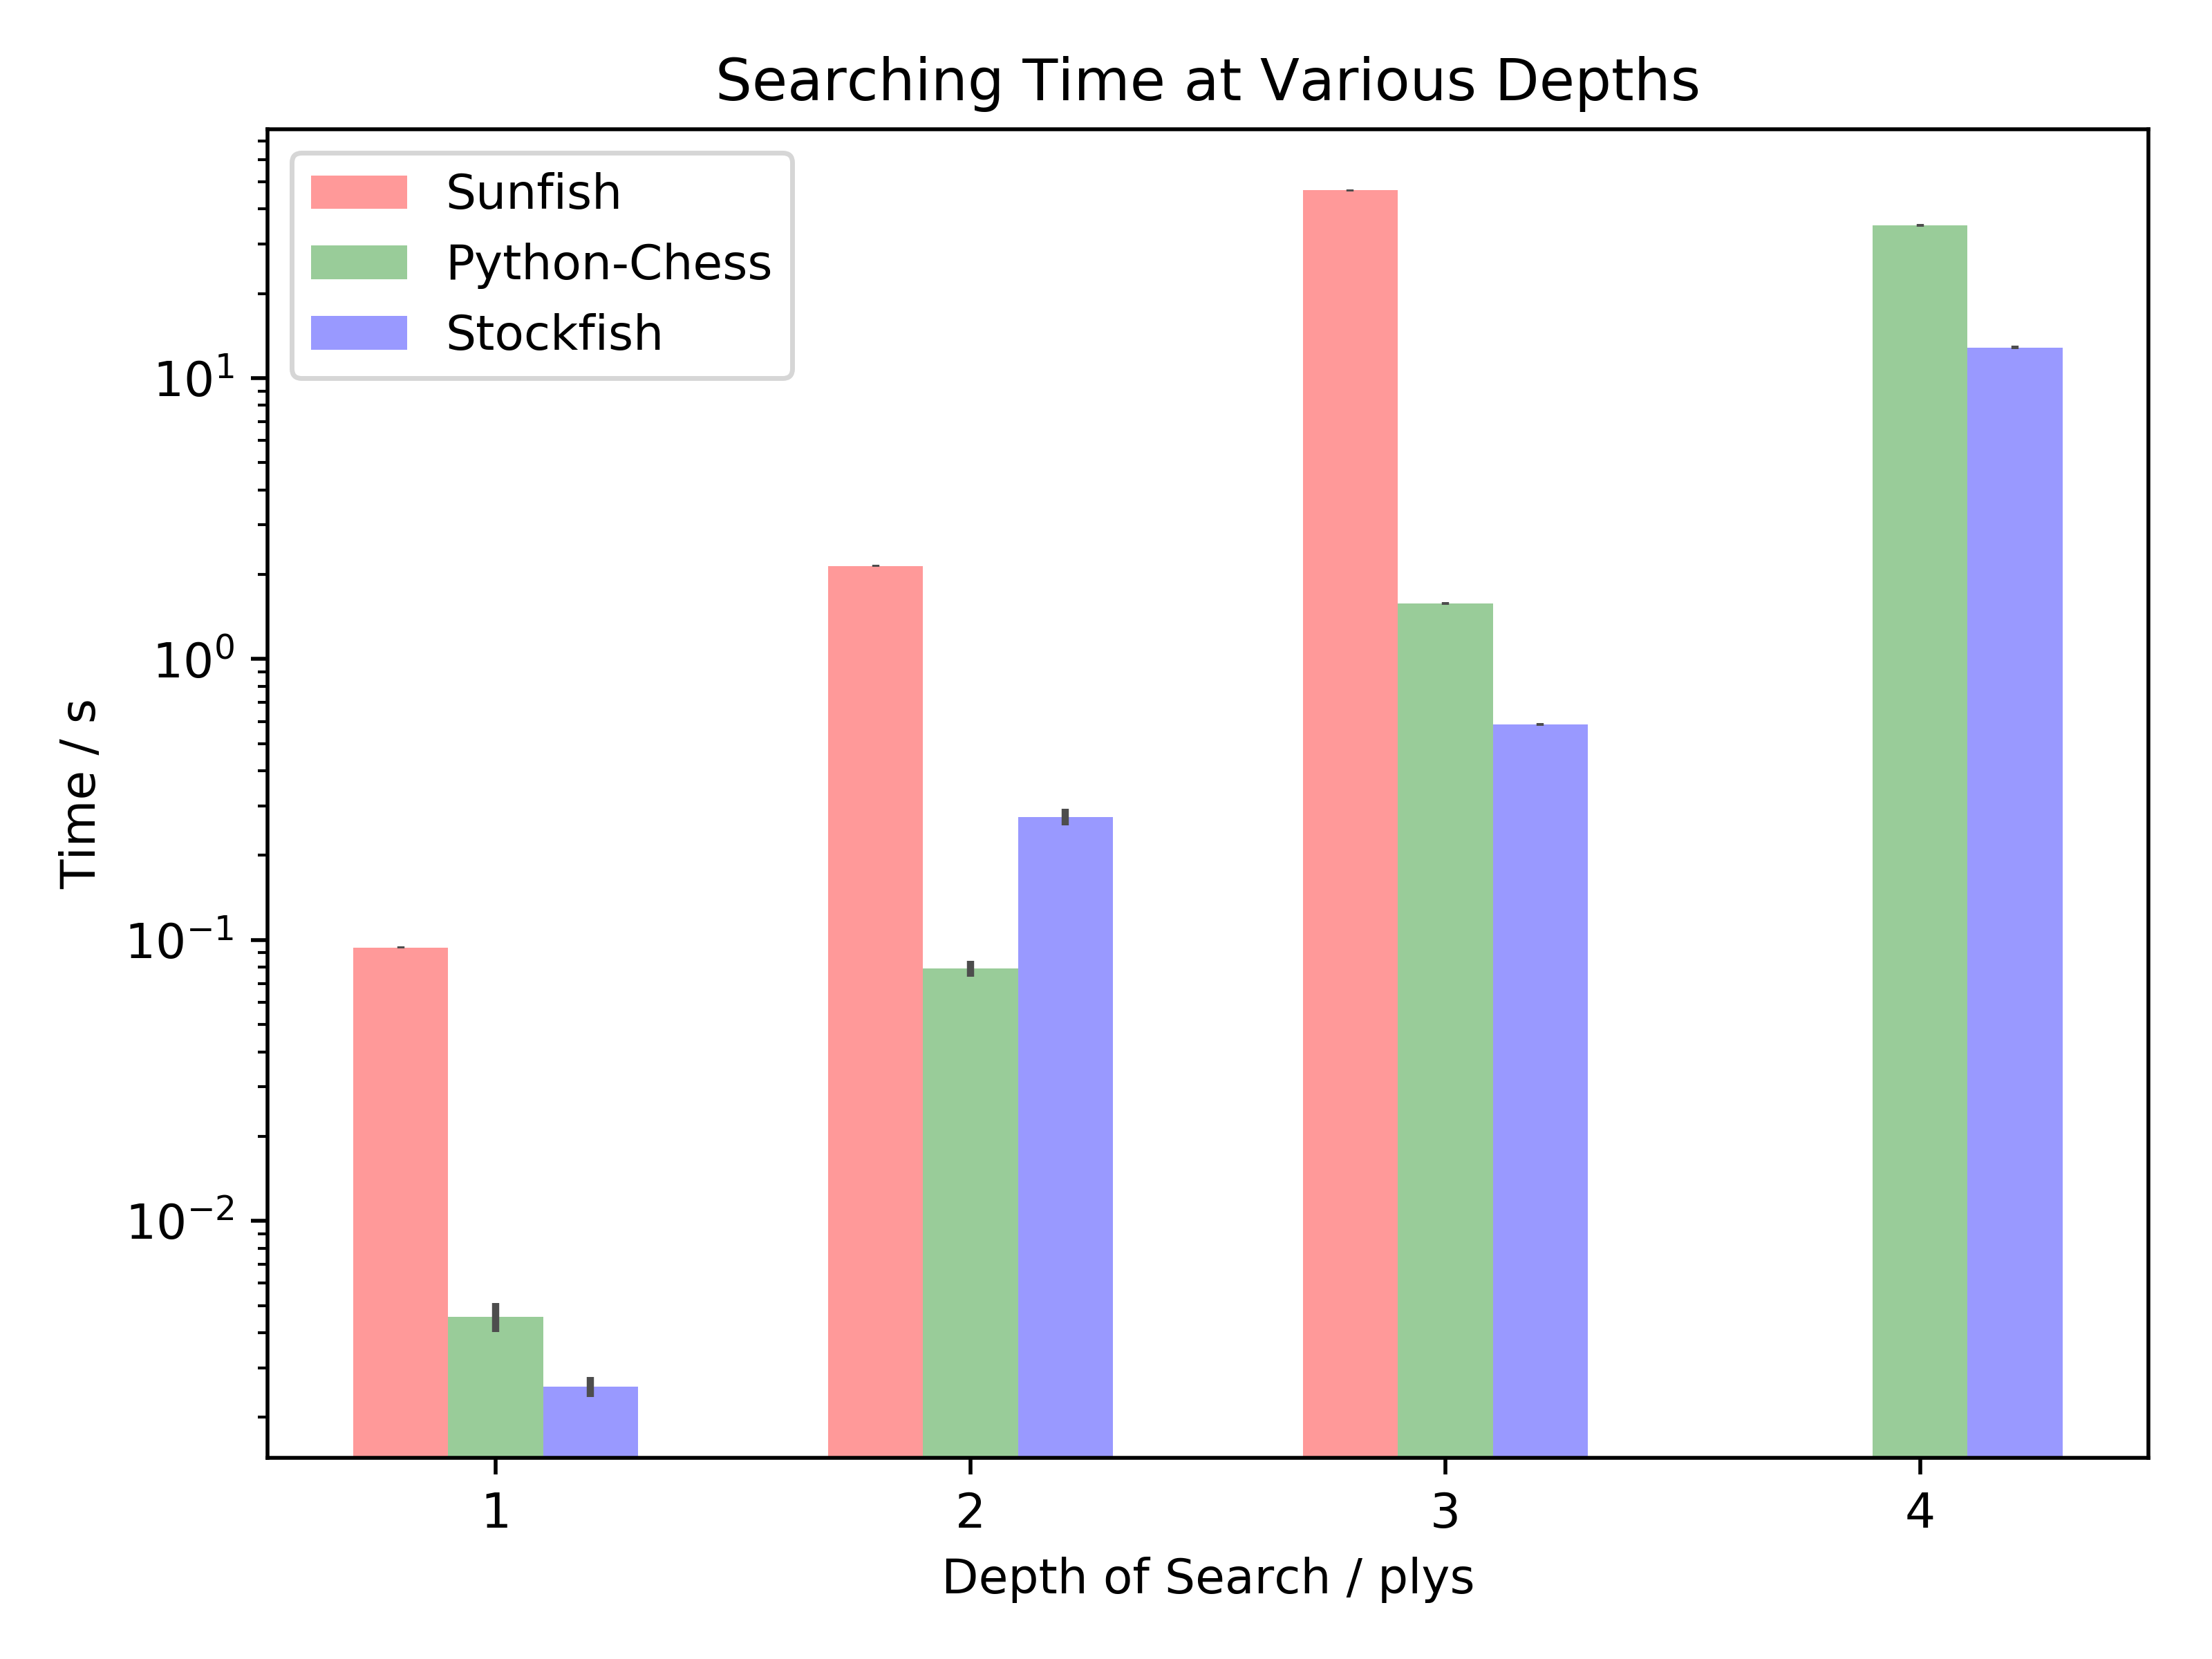
\includegraphics[scale=0.8]{movegenspeed.png}
\end{center}

\paragraph{} This confirmed the premise that for deeper searches, Stockfish was fastest and Sunfish slowest. Searching to a depth of 5 plys, or 4 in the case of Sunfish would have taken too much time. It is anticipated that the pruning heuristics would be able to speed up search even more. The scale factor of around 20 between times of successive plys confirm the fact that 20 is the average branching factor.

\paragraph{} As the speed of Stockfish and \texttt{PyTorch} has thus been shown, the next step would be to implement a search algorithm in \texttt{C++} which can train and use the \texttt{PyTorch} neural network as an evaluation function. Now that the prototyping phase has ended, the final codebase can be written and deployed in in \texttt{C++} for speed and efficiency.

\subsection{Inter-Process Communication between \texttt{Python} and \texttt{C++}}

\paragraph{} One of the first tasks was to embed \texttt{Python} in \texttt{C++} such that the neural network could be accessed with Inter-Process Communications (IPCs). Initially, a FEN string was passed from \texttt{C++} to \texttt{Python}. \texttt{Python} would convert it to the piecelist board representation, input it in the \texttt{PyTorch} neural network and return the output as a float. To improve the speed of this process, the board representation was created in \texttt{C++} and organised in \texttt{NumPy} memory format. A pointer to the array was passed to \texttt{Python}, which could pass the array to the network without any need for memory management. Correct implementation was ensured by checking that the network returned the same floating point. The overall process is presented in the following Message Sequence Chart.

\begin{center}
\begin{msc}{}
  \setlength{\instdist}{10cm}
  \declinst{C++}{}{\texttt{C++}}
  \declinst{Python}{}{\texttt{Python}}
  
  %\regionstart{activation}{Python}
  \regionstart{suspension}{C++}
  \mess{\textbf{1}}{C++}{Python}
  \nextlevel[2]
  
  \mess*{return list of functions}{Python}{C++}
  \regionend{C++}
  \regionstart{activation}{C++}
  %\regionend{Python}
  \regionstart{coregion}{Python}
  \nextlevel[3]
  
  \action{\textbf{2}}{C++}
  \nextlevel[3]
  
  \regionend{C++}
  \regionstart{suspension}{C++}
  \mess{\texttt{PyObject\_CallObject(py\_forward\_pass, representation)}}{C++}{Python}

  \regionend{Python}
  %\regionstart{activation}{Python}
  \action{\textbf{3}}{Python}
  \nextlevel[2]
  
  %\regionend{Python}
  \regionend{C++}
  \mess*{return floating point value}{Python}{C++}
  \regionstart{activation}{C++}
  \regionstart{coregion}{Python}
  \nextlevel
  
  \regionstart{coregion}{C++}
  \nextlevel[3]
  
  \regionend{Python}
  \regionend{C++}
  \mess{\texttt{Py\_Finalize()}}{C++}{Python}
\end{msc}
\end{center}

\begin{enumerate}
\item \texttt{Python} is embedded in \texttt{C++} when an interpreter session is started. The \texttt{PyTorch} neural network module is imported. A list of function pointers is returned to \texttt{C++}, enabling them to be accessed.
  \begin{verbatim}
    Py_Initialize();
    PySys_SetArgv(argc, argv);
    PyObject* module = PyString_FromString(``<path/to/network/file>'');
    PyObject* valueNetwork = PyImport_Import(module);
    PyObject* functions = PyModule_GetDict(valueNetwork);
    PyObject* fp = PyDict_GetItemString(functions, ``forward_pass'')
  \end{verbatim}

\item When a position is ready for evaluation, it is converted into a \texttt{NumPy} array \texttt{input}. A pointer to its memory location is passed into the function \texttt{fp}, returning a reference to an output float. \texttt{Py\_DECREF()} frees memory.
  \begin{verbatim}
    PyObject* output = PyObject_CallObject(fp, input);
    double d = PyFloat_AsDouble(output);
    Py_DECREF(output);
  \end{verbatim}
  
\item \texttt{fp} performs a forward pass of the \texttt{PyTorch} neural network.
  
\end{enumerate}

\paragraph{} IPCs for training the network follows the same framework, but with the weight update function instead of \texttt{forward\_pass}. To verify that it was correctly implemented, the agent was trained to play the KRvK endgame and the optimal value observed.

\subsection{Alpha-Beta Pruning Negamax with Transposition Tables}

\paragraph{} The Stockfish codebase contained an implementation of the Negamax algorithm, heavily optimised with 27 pruning heuristics. For simplicity, Negamax was reimplemented with alpha-beta pruning, move ordering and a transposition table. Alpha-beta pruning and move ordering was implemented from scratch, but Stockfish methods for accessing the transposition table, such as Zobrist hashing, was reused. To verify Negamax, Minimax without any pruning heuristics was also implemented. Stockfish's evaluation function was ported to \texttt{C++} and used to compare the output of Negamax and Minimax with the \texttt{Python} Negamax implementation.

\paragraph{} This was the last key component to be implemented. Following its implementation, the agent could then be trained on the full chess game. The remainder of the implementation time was spent on tuning hyperparameters and investigating how different board representations and architectures affected engine performance. Due to the similar scores of bitboard and piece-list representations described in Section 2.3.1, neural networks utilising both representations were explored. 

\subsection{Training and Tuning Hyperparameters}

\paragraph{} The two parameters to be tuned were $\alpha$ and $\lambda$. Out of the two, training was more sensitive to $\alpha$. When training on the KRvK endgame, the parameters were adjusted to observe their effect on the learning rate. The value of $\alpha$ fas first set as low as possible, before being gradually incremented to 0.01, the largest stable value of $\alpha$ where convergence of loss is observed. As training was not very sensitive to $\lambda$, a standard value of 0.7 was used.

\paragraph{} The effectiveness of altering the hyperparameters was observed by playing 100 games against a random agent. Other hyperparameters which affected training was the search depth of Negamax and the number of plys each game lasted. While the number of plys in a game used for evaluation was 80, training was improved if the number of plys in a training game was more than 80. As agents became stronger, there would not be a winner within 80 plys, and the reward signal returned to the agents would be 0. By increasing the number of plys, the occurrence of -1 and 1 in the reward signal increased, enabling the agent to learn how to win and lose, rather than draw. After trial and error, the optimal depth for this value is 160 plys. Any more plys would only yield diminishing rewards in the face of an attenuated training time.

\subsection{Piece Square Tables}

\paragraph{} Many chess engines such as Sunfish utilise piece square tables in their evaluation function. This is a vector of positive integers whose inner product with a bitboard chessboard representation returns a value. This computation can be achieved by running a single neuron with $bias = 0$ and a linear activation function. This network architecture is known as the piece square table.

\paragraph{} When finding a move, Sunfish evaluates the following expression using the evaluation function $f$. $\textbf{x}^{-1}$ is a flipped board representation which rotates a board by $180^o$ and swaps white pieces for black and vice versa.

\begin{align*}
  score &= f(\textbf{x}) - f(\textbf{x}^{-1}) \\
        &= w \cdot \textbf{x} - w \cdot \textbf{x}^{-1} \\
        &= w \cdot (\textbf{x} - \textbf{x}^{-1}) \\
\end{align*}

\paragraph{} The above expression simplifies the expression to one inner product and a subtraction. As Sunfish uses a bitboard board representation, $\textbf{x} - \textbf{x}^{-1}$ is thus equivalent to the antisymmetric bitboard described in Sectino 3.2.1. Thus the piece square table architecture consisting of a linear combination of an antisymmetric bitboard and weight vector was implemented in \texttt{C++} and trained with TD($\lambda$) and TD-Leaf($\lambda$).

\subsection{Overview of Final Codebase}

\paragraph{} The implemented components was a chess engine, reinforcement learning algorithms and an agent which played randomly selected moves. A UML class diagram of the final codebase is shown below.

\begin{center}
  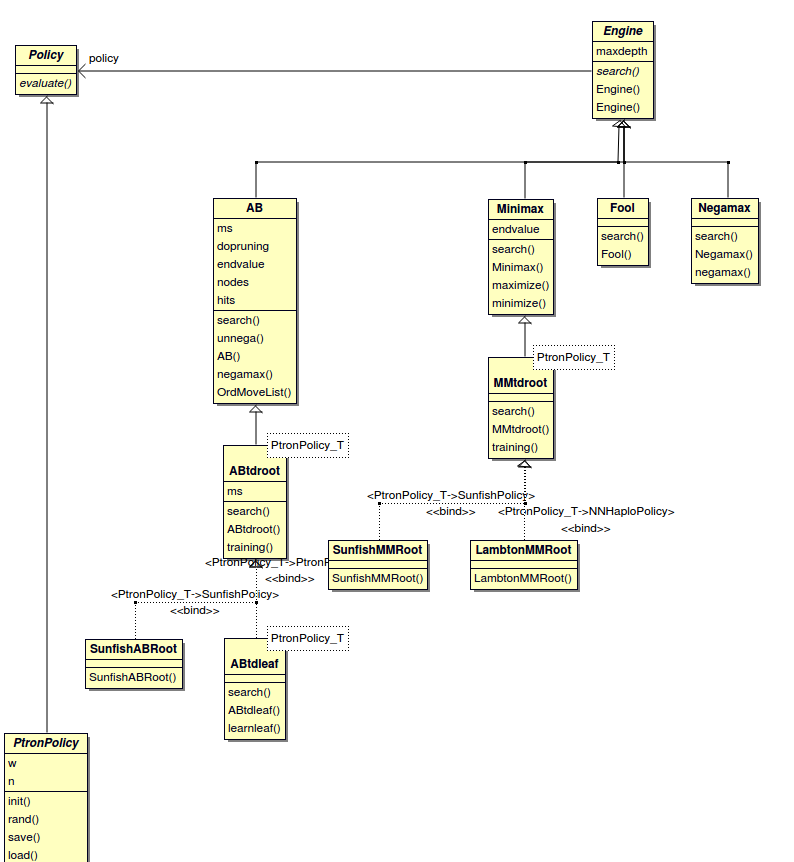
\includegraphics[scale=0.4]{umlClass.png}
\end{center}


\paragraph{} The main class in the final codebase is Policy. This class is used to find the best move given a chessboard position. It has an Engine which is responsible for searching and evaluation. PtronPolicy is the simplest policy of all, and is an implementation of a perceptron in \texttt{C++}.

\paragraph{} Engine is a class which can be AB (alpha-beta), Minimax, Negamax or Fool (an agent playing a random move). As AB is used in training, it can be ABtdroot (TD($\lambda$)) or ABtdleaf (TD-Leaf($\lambda$)), depending on which training algorithm is used. This, as described, utilised the SunfishABLeaf (Sunfish piece square tables) as an evaluation function.

\paragraph{} For debugging, Minimax was used to verify that AB gave correct evaluations. It has two interchangeable policies, Sunfish and Lambton MMRoot (standing for MiniMaxRoot). SunfishMMRoot was another implementation of the Sunfish piece square tables, whereas lambton is the Medium Network written in \texttt{PyTorch}, so called because The Lambton Worm was a snake (\texttt{Python} is a snake) which lived in water. There has been a longstanding tradition of chess engines named after fish.

\paragraph{} The following template heirarchy illustrates how various policies were derived from a perceptron.

\begin{center}
  \includegraphics[scale=0.6]{umlTemplate.png}
\end{center}

\paragraph{} Finally, the NNpolicy (Neural Network Policy) is a supertemplate of NNHaploPolicy, used to interface with the \texttt{PyTorch} neural network. This policy is so named because the Haplochromine fishes are bright and luminous, like torches.

\begin{center}
  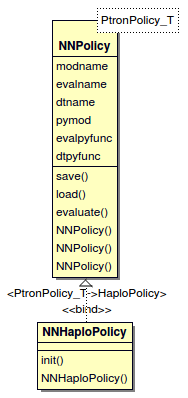
\includegraphics[scale=0.6]{umlPolicyTemplate.png}
\end{center}

%\paragraph{} Much fun was derived from the nomenclature of the classes.

%\section{TreeStrap Learning Algorithm, an Extension}

%\paragraph{} Although implementing TreeStrap was more straightforward than TD-Lambda and TD-Leaf, the majority of time in development was spent in verifying TreeStrap and using it to successfully train an agent. Research has concluded that TreeStrap is highly unstable and prone to overfitting. This causes a significant decrease in playing ability. To mitigate the effects of overfitting, modifications published later by one of the co-authors was combined with a heuristic adapted from KnightCap. Other proposed modifications to TreeStrap were deemed too numerous and time-consuming to explore, and is left as a possible research direction to the interested reader.

\section{Conclusion}

\paragraph{} The chapter presents an insight into the project's implementation. Following a fruitful exploration, experiments regarding board representation, network architecture and training on a chess subproblem were undertaken in stage 2. In stage 3, Stockfish was modified to use a \texttt{PyTorch} neural network with a custom loss function and weight updater.

%\paragraph{} An unforeseen complication arose when writing the loss function and weight updater in \texttt{PyTorch}. To the best of the author's knowledge, no equation for the loss function of TD learning has been written. Some time was spent deriving the expression and showing that it computed an equivalent value to equations for the weight updater expected literature. This was complicated by the fact that the equation for weight updating was written incorrectly in some papers.

%\paragraph{} Nevertheless, a chess agent and deep reinforcement learning methods were implemented and trained. The results are analysed in the next section.

\chapter{Evaluation}

\paragraph{} In the previous chapter, evaluation of some components such as the board representation, network architecture and hyperparameter values were undertaken during implementation, such that they can be used to guide the implementation process. This chapter evaluates of the final codebase and trained agent, and explains why the examinable objective has been achieved. First, an empirical evaluation of the examinable objective is presented, before its validity and reproducibility is analysed in summative evaluation.

\section{Objective}

\paragraph{} The examinable objective was declared in the form of a null and alternate hypothesis. The goal of the project was to show that there is no reason to reject the alternate hypothesis to 95 \% significance.

\paragraph{Null Hypothesis:} Within a chess game of 80 plys, there is no significant difference between a trained agent and one that plays randomly generated moves.

\paragraph{Alternate Hypothesis:} Within a chess game of 80 plys, a trained agent performs better than one that plays randomly generated moves.

\paragraph{} To compute significant difference, the win ratio of a trained agent to a random agent was compared against two random agents playing against each other.

\subsection{Win Ratio of Agent Trained by TD($\lambda$)}

\paragraph{} When two random agents played against each other, the win ratio was consistently 0 \%, because it was very unlikely that a random walk leads to checkmate. This number was confirmed by counting the number of wins in 10 batches of 100 80-ply games.

\paragraph{} A piece square table architecture of an evaluation function was trained on 500 games of self-play using TD($\lambda$). Hyperparemeters used were derived from experimentation as mentioned in the previous chapter.

\begin{center}
  \begin{tabular}{c | c }
    \hline
    \textbf{Hyperparameter} & \textbf{Value} \\ \hline
    $\alpha$ & 0.01 \\
    $\lambda$ & 0.7 \\
    Negamax Search Depth & 4 \\
    Training Ply Cutoff & 160 \\
    Initial Random Plys & 4 \\
    \hline
  \end{tabular}
\end{center}

\paragraph{} After every 50 games of self-play, 100 games were played against the random agent. The graph shows the cumulative wins in these 100 games vs the ply at which the win was achieved. The win ratio for a trained agent against a random agent could be as high as 84 \%. 

\begin{center}
  \centerline{Cumulative Win \% of Agent Trained by TD($\lambda$) vs End Ply}
  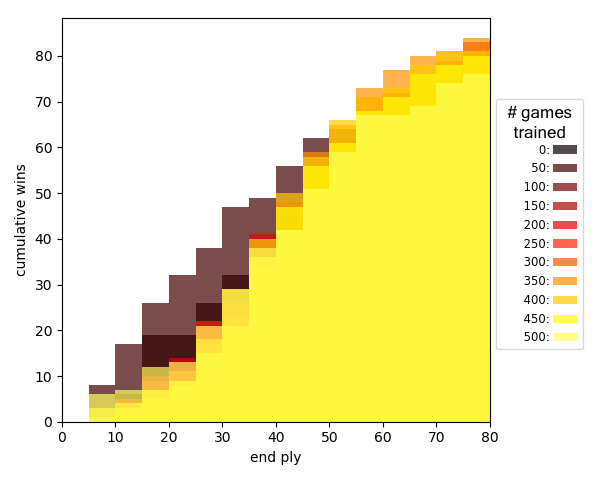
\includegraphics[scale=0.5]{lambdahist2.png}
\end{center}

\paragraph{} The emerging sigmoidal shape of the cumulative wins graphs indicates that the agent is overfitting to playing against itself. In supervised learning with a training and evaluation set, overfitting means the machine learning model is learning features locally specific to the training set which are not present in the underlying distribution. This would reduce the accuracy of evaluation. Overfitting is particularly prevalent in large neural networks with plenty of neurons.

\paragraph{} Although the piece square table architecture -- a single neuron -- would not overfit in supervised learning, this can occur in reinforcement learning. Instead of learning general strategies, the agent is overfits and learns how to play against itself. Preventing overfitting in reinforcement learning is more challenging than in supervised learning because the online nature of reinforcement learning algorithms generate data depending on the behaviour of the agent, rather than having a constant underlying distribution. The emerging sigmoidal shape is indicative of overfitting because the agent learns how to play more effectively towards 60 -- 80 plys, and forgets how to win from 10 -- 40 plys. The ideal shape of the graph is linear with a gradient of 1, because the agent should be equally likely to win at any ply, given that the opponent is a random agent and will not change strategy based on the point at the game. This shows that instead of learning how to play the same game with the same moves or the same strategies, the agent is capable of identifying a checkmate situation and exploiting it. 

\paragraph{} By averaging the values of 10 batches of 100 games against a random agent, 95 \% confidence intervals were calculated. 

\begin{align*}
  \overline{x} \pm 1.96 \times \frac{\sigma}{\sqrt{n}} = 73 \text{ to } 79.8 \%
\end{align*}

\paragraph{} As 0 was not in the range of this interval, there is no reason to reject the alternate hypothesis. Hence the criteria of the project has been met. When the Negamax search depth was reduced to 2, the peak win ratio was reduced from 84 \% to 76 \%, as illustrated in the following graph.

\begin{absolutelynopagebreak}
\begin{center}
  \centerline{Cumulative Win \% of Agent Trained by TD($\lambda$) vs End Ply}
  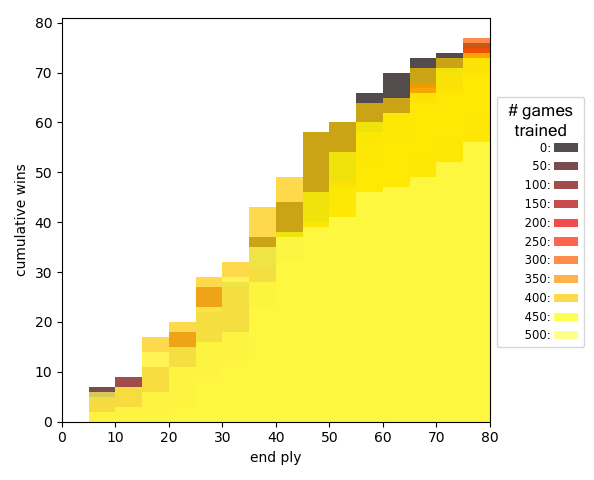
\includegraphics[scale=0.5]{lambdagood.png}
\end{center}
\end{absolutelynopagebreak}

\paragraph{} This shows that the depth of search only marginally affects the overall performance of the agent when trained by TD($\lambda$). An extreme of overfitting is presented in the following graph, generated from the same training conditions as the graph above but with a different weight initialisation.

\begin{absolutelynopagebreak}
\begin{center}
  \centerline{Cumulative Win \% of Agent Trained by TD($\lambda$) vs End Ply}
  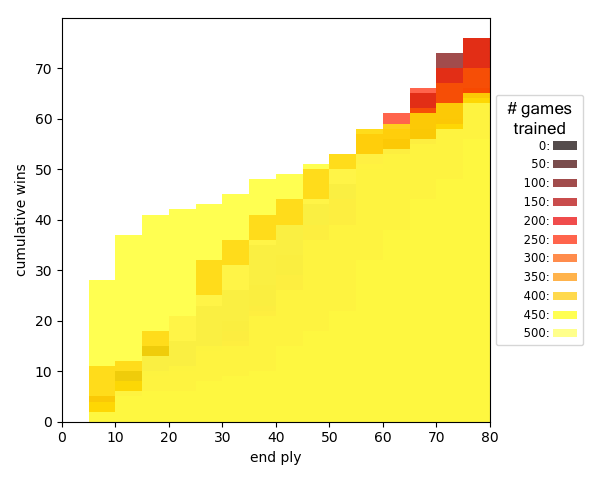
\includegraphics[scale=0.5]{lambdabad.png}
\end{center}
\end{absolutelynopagebreak}

\paragraph{} In this graph, the network overfits and learns strategies which are more effective when the plys are 0 -- 40, at the expense of learning strategies later on in the game. This is the opposite of the sigmoidal cumulative curve shown in previous graphs.

\subsection{Win Ratio of Agent Trained by TD-Leaf($\lambda$)}

\paragraph{} The agent was trained for 500 games of self-play using TD-Leaf($\lambda$). The following graph shows the cumulative wins in the batch of 100 games vs the ply at which the win was achieved, for every 50 games of self-play.

\begin{absolutelynopagebreak}
\begin{center}
  \centerline{Cumulative Win \% of Agent Trained by TD-Leaf($\lambda$) vs End Ply}
  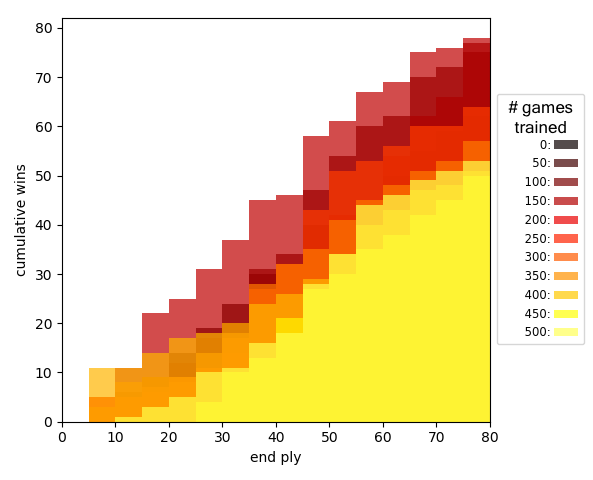
\includegraphics[scale=0.5]{leaf.png}
\end{center}
\end{absolutelynopagebreak}

\paragraph{} As the maximum win ratio of 75 \% was rather similar to the value generated by training with TD($\lambda$), this could imply that training of this network architecture cannot be improved any further. To improve the power and capacity of the value network, a larger network should be used. Overfitting was more severe in TD-Leaf($\lambda$) than TD($\lambda$), implying that TD-Leaf($\lambda$) is a stronger learning algorithm.

\paragraph{} However, results obtained through training the Medium Network using TD($\lambda$) and TD-Leaf($\lambda$) yielded similar results to those presented above. It is possible that some bugs remain, preventing the network from training efficiently. Due to time constraints, these had not been fully debugged.

\subsection{Reproducibility}

\paragraph{} To show that the results were reproducible, the weights of the value network were initialised to different random values. The agent was then trained for 1100 games, at which point the win ratio started to decrease because the neural network was overfitting.

\begin{absolutelynopagebreak}
\begin{center}
  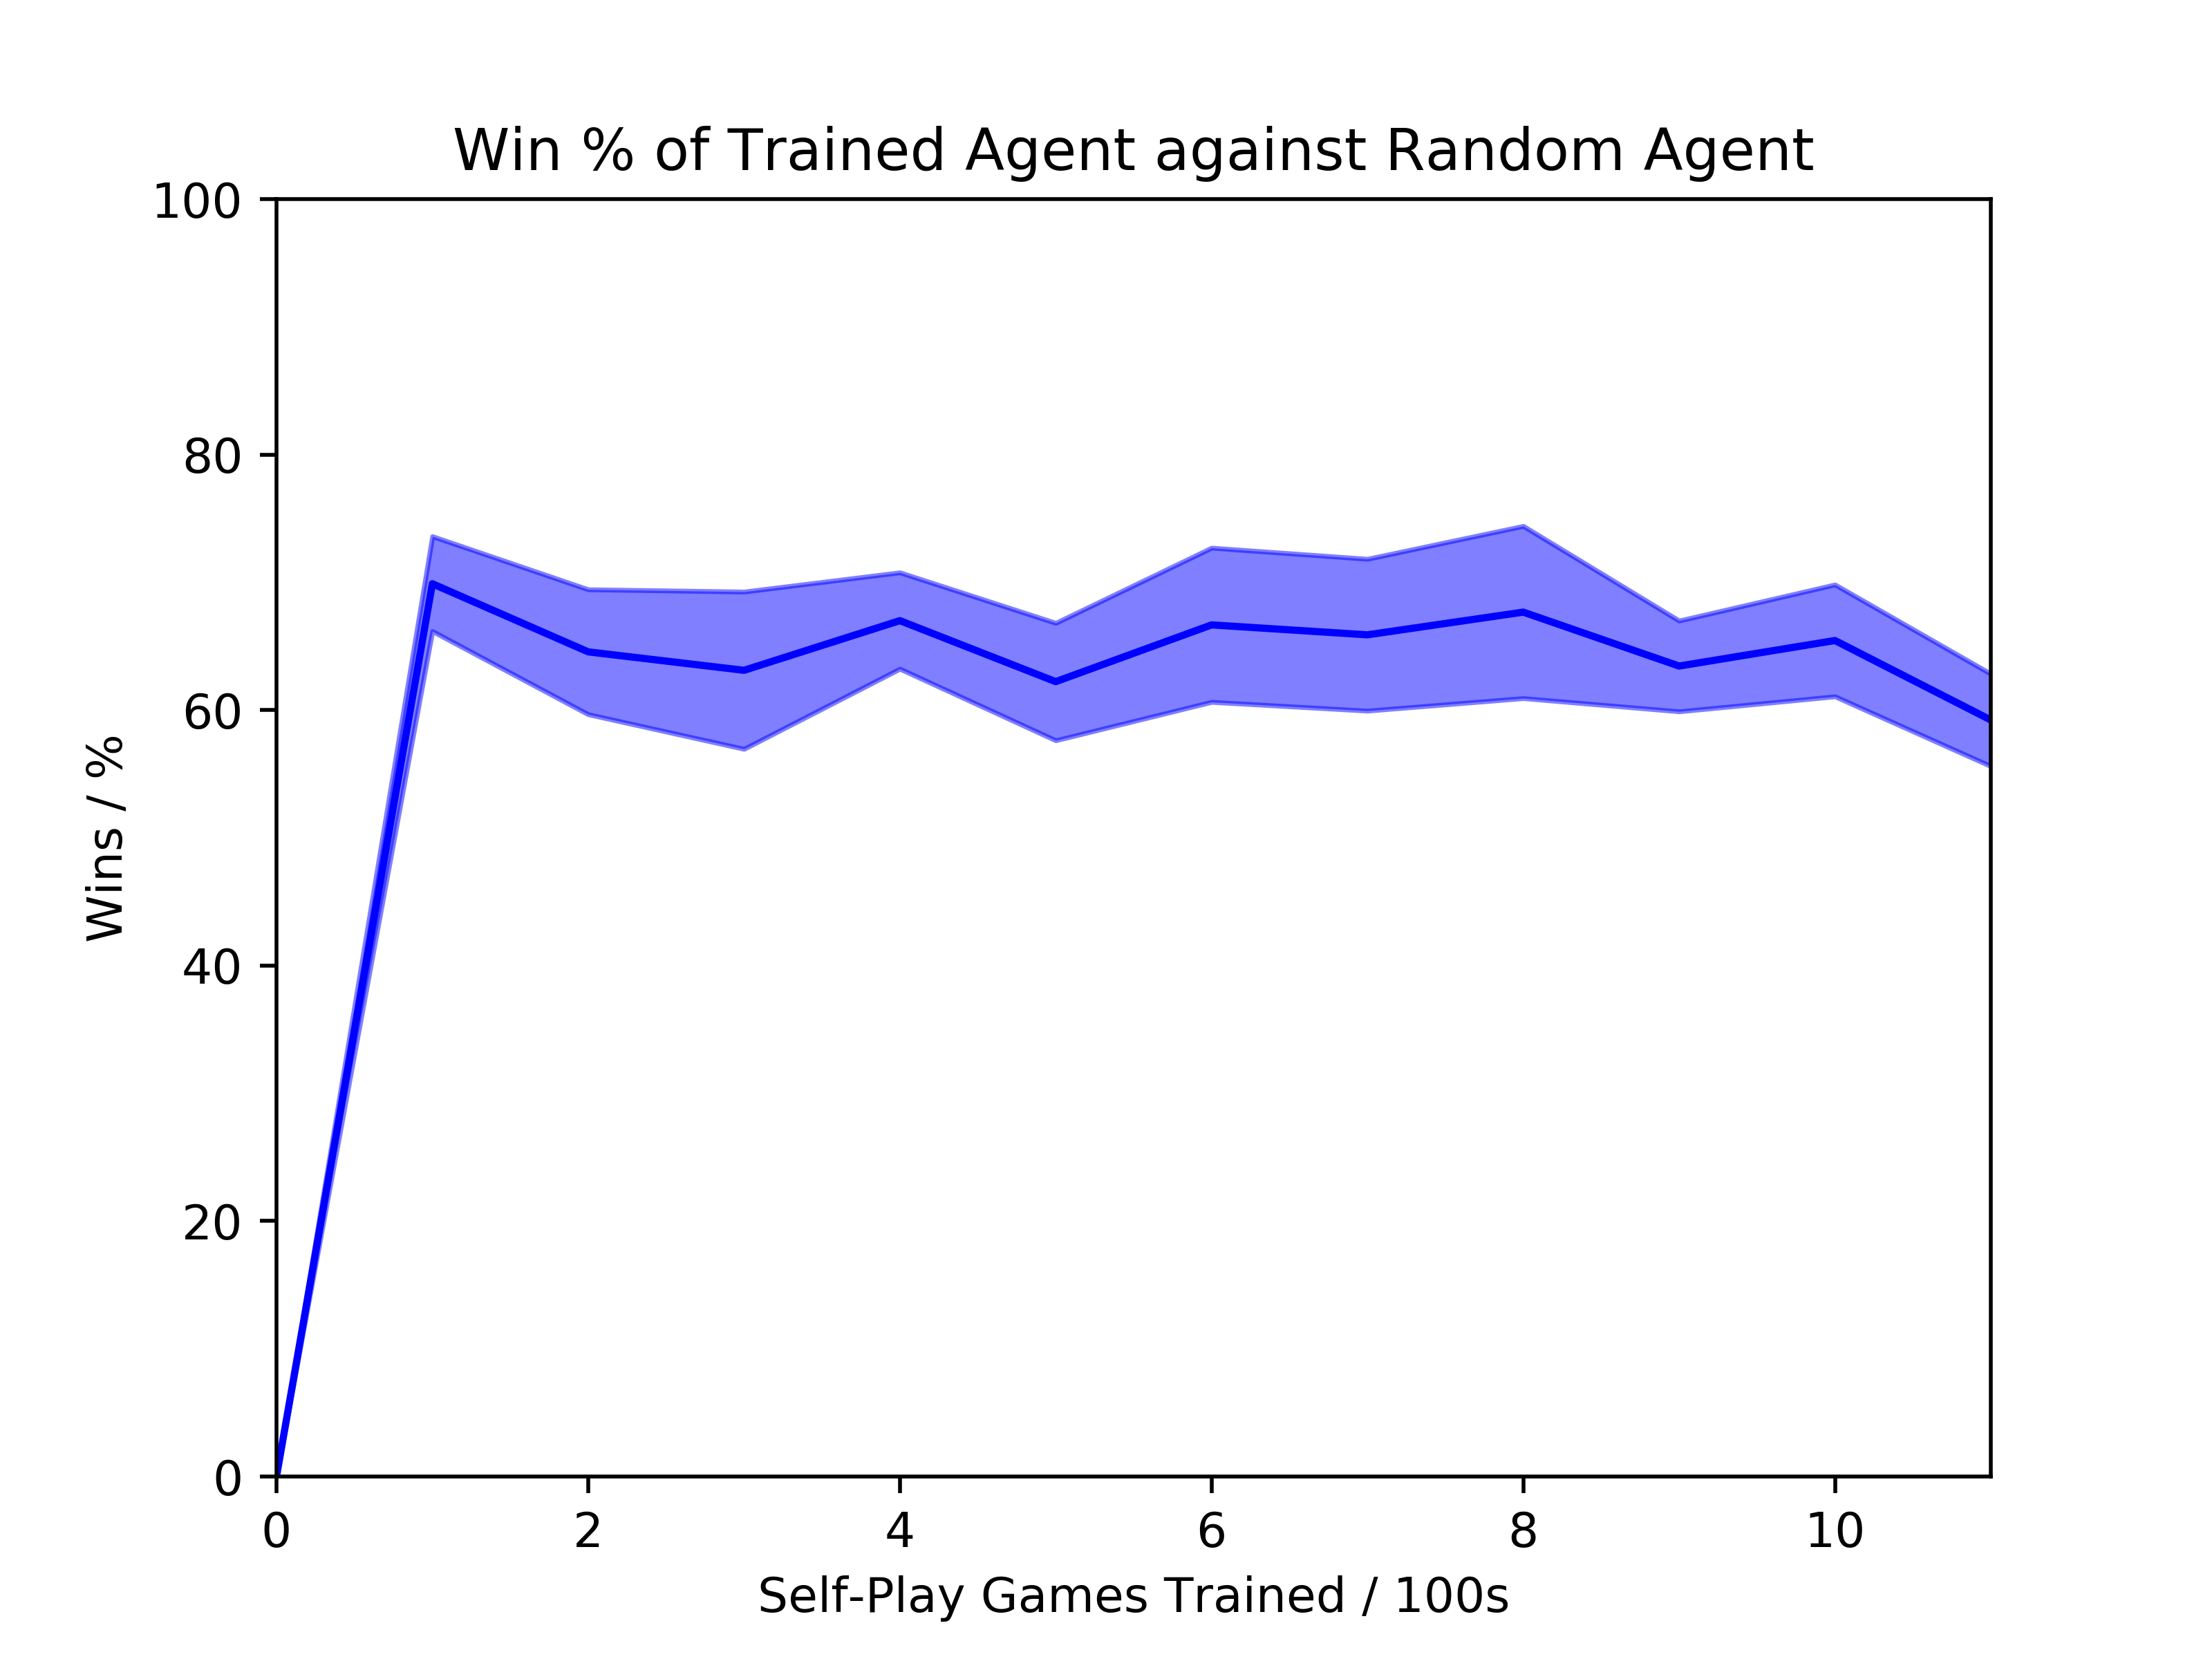
\includegraphics[scale=0.75]{winsreproducelambda.png}
\end{center}
\end{absolutelynopagebreak}

\paragraph{} Overfitting occurred because the agent is becoming better at playing against itself but not against a random agent. This can be combatted by increasing exploration to vary the games the network is being trained on. During self-play, the first four moves were randomly selected, enabling the agent to explore various games. By increasing this value, the agent could be trained with a greater amount of exploration.

\paragraph{} The same graph for an agent trained with TD-Leaf($\lambda$) is presented below.

\begin{absolutelynopagebreak}
\begin{center}
  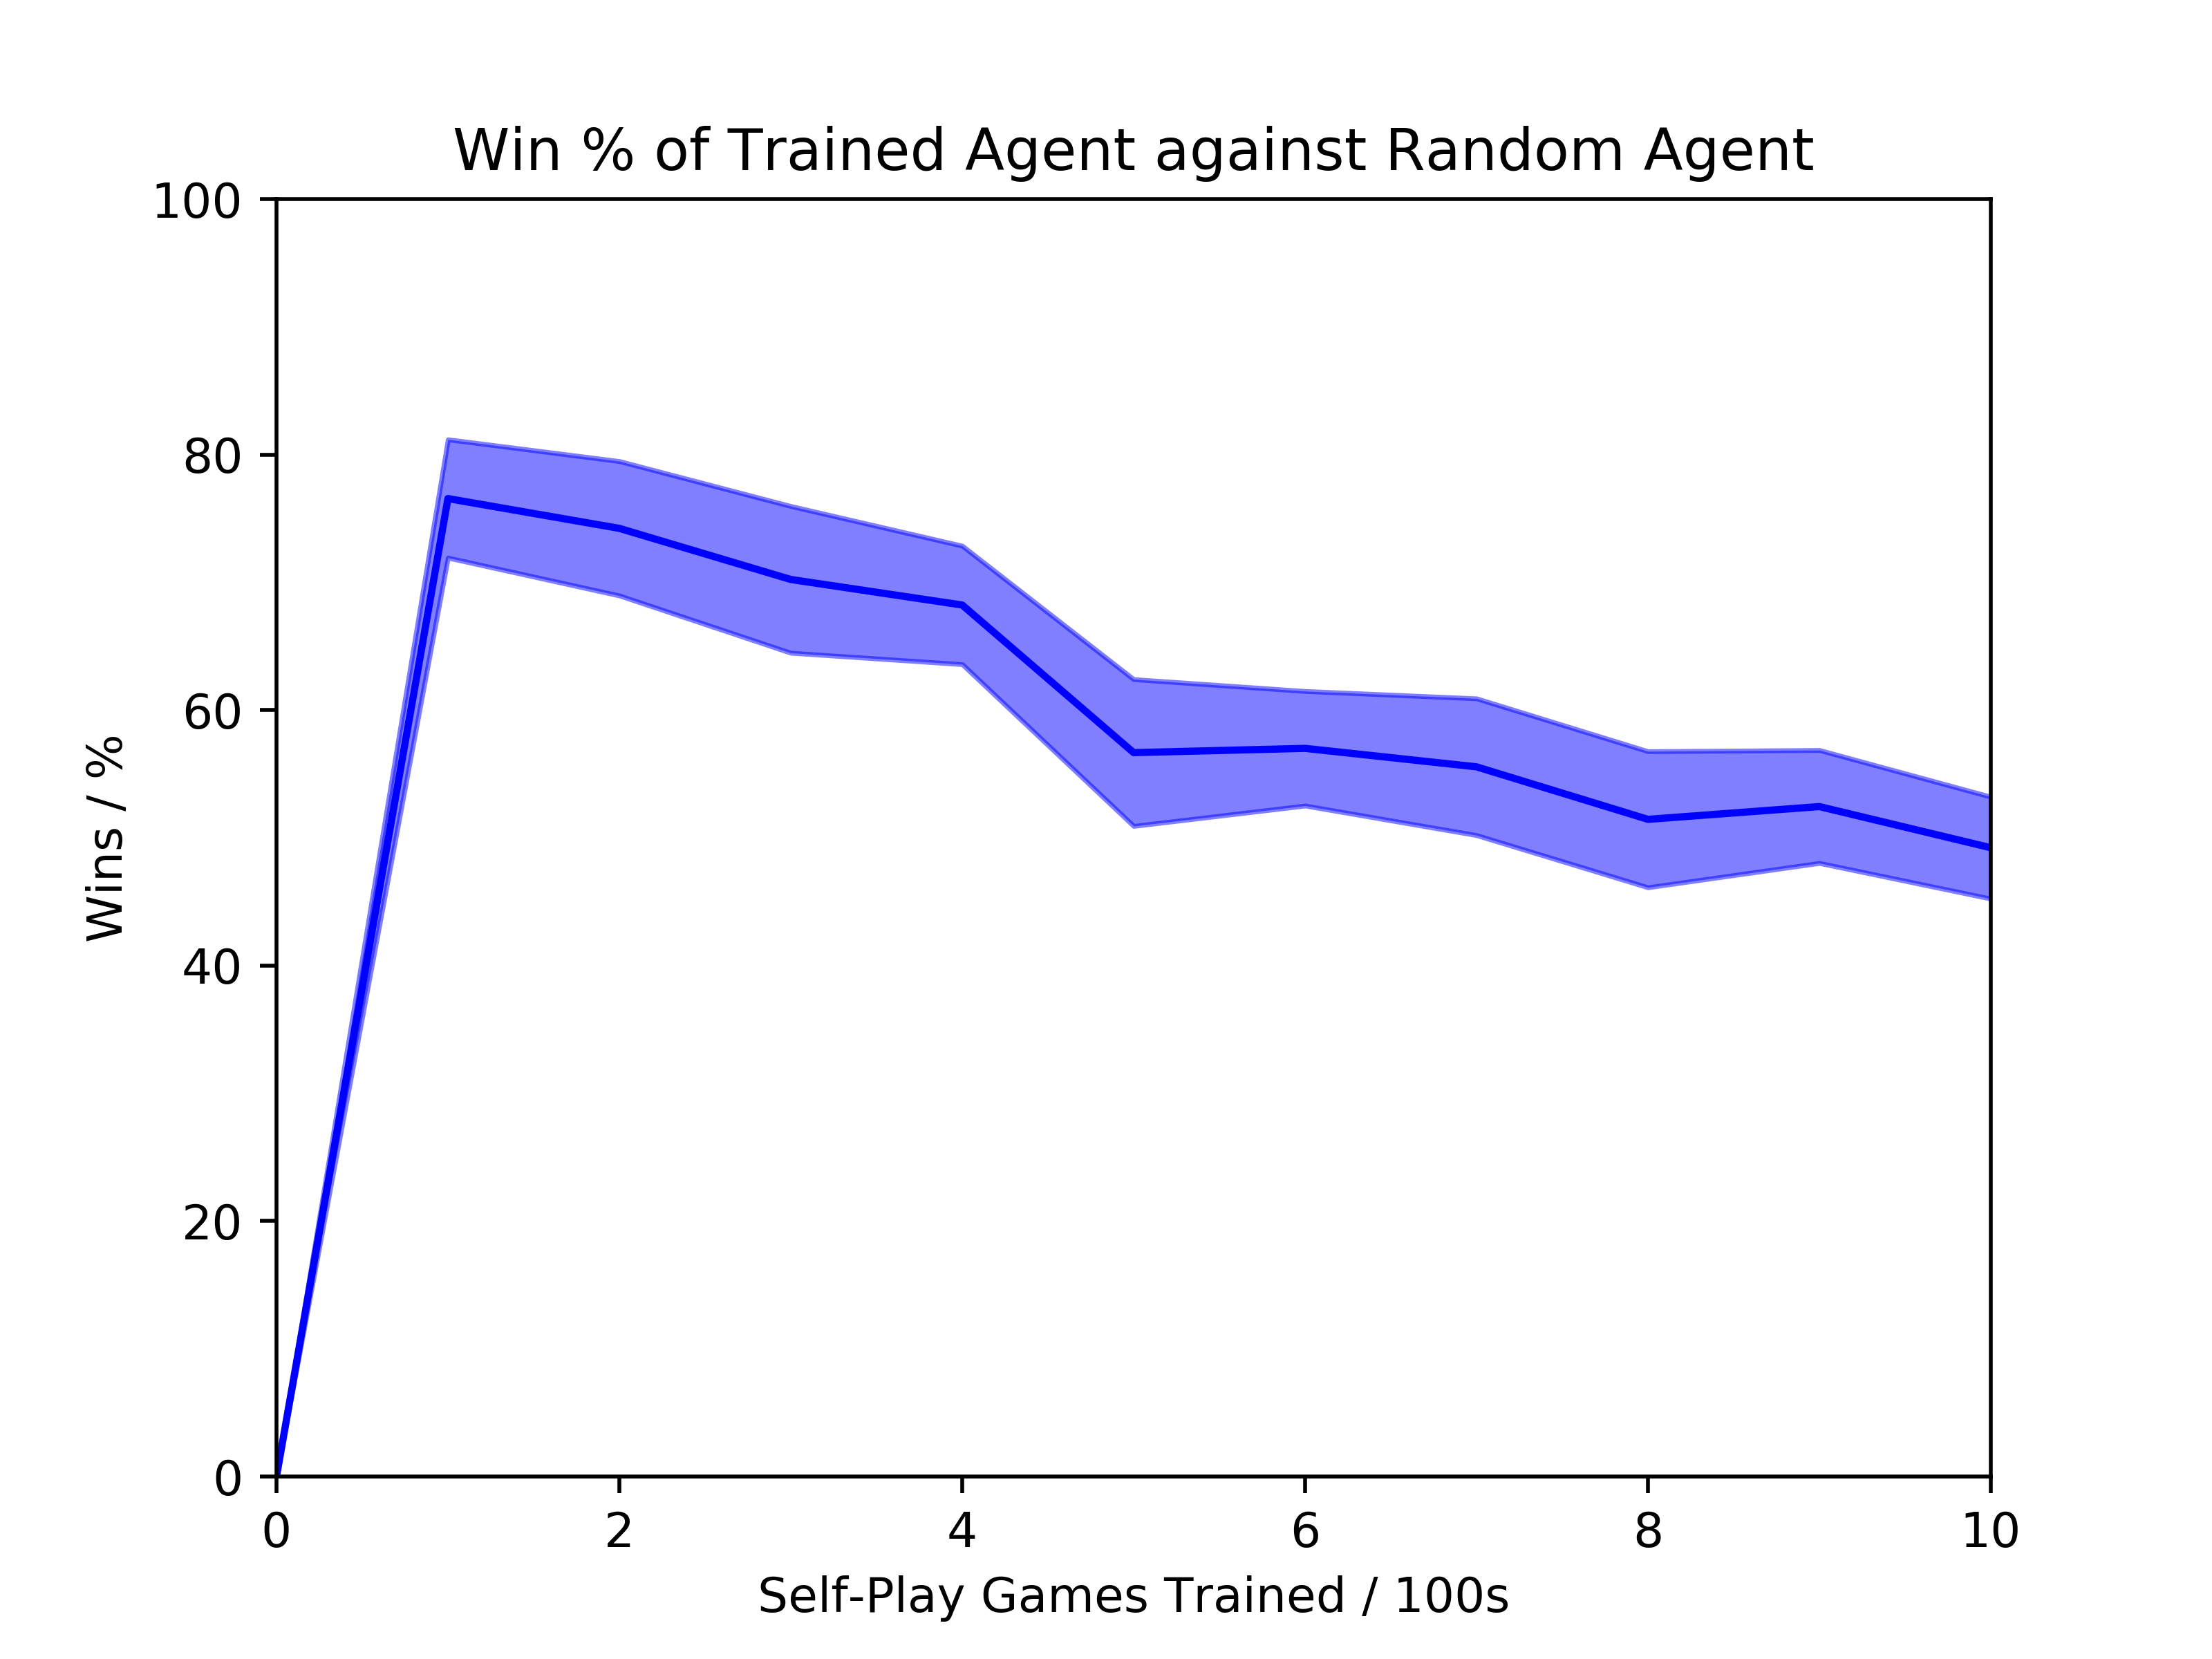
\includegraphics[scale=0.75]{winsreproduceleaf.png}
\end{center}
\end{absolutelynopagebreak}

\paragraph{} As TD-Leaf($\lambda$) was a more powerful training algorithm, it overfitted more quickly. Hence the decline in win rate is accentuated more for the graph produced by TD-Leaf($\lambda$).

\section{Summary}

\paragraph{} This chapter shows that the objective has been successfully met, and confirms initial results in the Implementation chapter that TD-Leaf($\lambda$) is a stronger training algorithm than TD($\lambda$). Evaluation of individual components of the chess engine have been presented in the Implementation chapter, because results from these evaluations shaped the structure of the resultant chess engine. %such as finding a board representation, hyperparameter values, and cascade correlation 

\chapter{Conclusion}

\paragraph{} Overall, this dissertation describes how a chess engine can be trained using deep reinforcement learning. A novel board representation only encoding piece coordinates was used, as well as a new network architecture. The results were a success, fulfilling the requirements of the examinable objective. In addition, the agent was trained by self-play with minimal human knowledge, making this project one of the few chess agents trained in this way. This project also showed that it was possible to train chess agents on commercial hardware.

\paragraph{} Although the agent did not attain superhuman performance, it learned the relative value of pieces and was significantly stronger than a random agent, fulfilling the core objective. With a longer training time and larger network, the agent's strength would increase, perhaps leading to better performances.

%\paragraph{} Having had no experience with programming a chess agent before, the author feels that, in addition to learning about reinforcement learning and deep learning, plenty of knowledge was learnt about chess and programming practices. This was the largest coding project attempted by the author, and was much more challenging than anticipated.

\section{Lessons Learned}

\paragraph{} The most challenging component of the project was getting the search algorithm to run at an adequate speed. This was achieved by adapting the move generator in \texttt{Stockfish} in a searching algorithm. This reimplemented the search algorithm which had already been written in \texttt{Python}. Time could have been saved by implementing the search algorithm directly in \texttt{C++} without using \texttt{Python}.

\paragraph{} Although easy to implement, cascade correlation took a long time to run. As the strength of the final agent did not depend much on the network architecture, this step would not have been necessary.

%\paragraph{} An invaluable lesson learnt when dealing with machine learning problems is to save the results of training and evaluation where possible, as it is very easy to overwrite and lose them. Furthermore, data should be saved to include as much detail as possible.

\section{Further Research Directions}

\paragraph{} An obvious next step would be to improve the efficiency of the final codebase and removing any lingering bugs such that deeper searching could be achieved with a larger neural network, increasing the strength of the agent.

\paragraph{} Compared to other chess engines, the evaluation function was implemented in \texttt{Python}. To increase speed, a possible research direction would be to reimplement neural networks in \texttt{C++}, reducing the need for IPC and increasing speed. In addition, multithreading could be used in searching, increasing the number of board positions evaluated per game.

%\paragraph{} Within the evaluation function, other network architectures could be examined, including convolutional and residual layers. A value network created with these layers may create more powerful representations, enabling a better approximation to the ideal evaluation function. This could be combined with other deep reinforcement learning algorithms such as TreeStrap or Sarsa($\lambda$).

\paragraph{} Deep learning has developed other loss functions and weight updaters. Rather than using the minimum squared error and stochastic gradient descent, the impact of using other methods could be investigated.

\section{Summary}

\paragraph{} Overall, learning about deep reinforcement learning and implementing its algorithms in chess has been a challenging but enjoyable experience. By building on the foundations of this project, there a lot of potential ideas for future research directions.
















\bibliography{giraffe} 
\bibliographystyle{plain}


\appendix

\chapter{Forsyth-Edwards Notation (FEN)}

\paragraph{} Forsyth-Edwards Notation (FEN) represents a chessboard as a string for easy storage. The starting position

\begin{center}
  \medskip
  \newgame
  \showboard
\end{center}

\paragraph{} is represented by \texttt{rnbqkbnr/pppppppp/8/8/8/8/PPPPPPPP/RNBQKBNR w KQkq - 0 1}

\paragraph{} There are six terms in a FEN, delimited by spaces.

\begin{enumerate}
\item The location of pieces are stored by their letter in a raster sequence, from a8 to h1.
\item The identity of the player to move.
\item Castling rights. White is represented in uppercase, and kingside castling is represented with K.
\item En passant square availability.
\item Number of plys since a pawn was last captured.
\item Number of full moves (equivalent to the number of moves black has taken)
\end{enumerate}
  
\chapter{Project Proposal}
\newpage
\centerline{}
\vspace{1in}
\centerline{\LARGE Computer Science Tripos, Part II, Project Proposal}
\vspace{0.2in}
\centerline{\large David Yu-Tung Hui, Trinity College}
\vspace{0.15in}
\centerline{\large October 20, 2017}
\vspace{0.3in}

\centerline{\huge Deep Reinforcement Learning For Chess}
\vspace{0.2in}
%\centerline{\large Combining Rule-Based Search Algorithms with Deep}
%\vspace{0.05in}
%\centerline{\large Reinforcement Learning in the Context of Chess}
%\vspace{0.45in}
\centerline{\large Originator: David Yu-Tung Hui}
\vspace{0.05in}
\centerline{\large Project Supervisor: Dr. Sean Holden}
\vspace{0.05in}
\centerline{\large Project Overseers: Dr. Markus Kuhn, Pr. Peter Sewell}

\section*{Introduction}

\paragraph{}Recent advances in Artificial Intelligence combine the strengths of two subfields to produce powerful hybrid agents. Such agent architectures include AlphaGo, the first computer program to play Go with superhuman ability. \cite{AlphaGo} By harnessing Deep Reinforcement Learning with classical search algorithms, hybrid architectures possess the advantages, as well as weaknesses, of both fields.

\paragraph{}To analyse such architectures, I will reimplement \textit{Giraffe}, a predecessor of AlphaGo. Developed by Matthew Lai, Giraffe was trained on a CPU in Chess, achieving a strength of an international master. \cite{giraffe} My reimplementation would run on a GPU, making it one of the first chess engines to do so. With the increasing cost-effectiveness of GPUs, speedups in Deep Learning are attained and are becoming more popular. However, they are rarely used in Chess because most agents rely on hand-crafted search and evaluation algorithms with no machine learning. Optional further extensions would modify the searching algorithm and conduct empirical user studies.

\paragraph{}Combining rule based algorithms with Deep Learning would unify many years of orthogonal research, and perhaps provide a foundation of the direction to come. It is possible that this new architecture may yield a new strategy within the game of Chess, enhancing the knowledge of the game as well as providing a new opponent for humans to train against.

\section*{Substance and Structure}

\paragraph{}The finished codebase will consist of an agent capable of playing against chess engines and humans using the GNUChess / XBoard Communication Protocol. Deep Learning networks run on top of an internal board representation, adapted from Giraffe. This contains rules and constraints on the legality of moves. Optional project extensions add another searching algorithm for comparison. In addition to the code, analysis of the above techniques will be summarised in the Dissertation.

\paragraph{}Giraffe is based around \textit{Probability-Limited Search}. From the current board position, a \textit{game tree} is created by simulating all possible games until the probability of principal variation dips below a threshold value. Principal variation occurs when the nature of the game changes, for instance between midgame and endgame, or in checkmate, when a player wins. \textit{Minimax} runs on the tree to find the optimal move. This is so named because the best move maximises the minimum values your opponent can force.

\paragraph{}Built around this are two \textit{deep neural networks}, the quality of which are the most important part of the project. One neural network evaluates the value of a board and is known as the \textit{value network}. The other estimates the probability of principle variation, generating the search tree. As Chess players have timed moves, these will have to be coded efficiently to search as many nodes as possible.

\paragraph{} There are two training phases. First, (board, distance-to-checkmate) pairs pre-train the value network by \textit{supervised learning}, where distance-to-checkmate is an initial approximation of value. During the second phase, the agent plays against itself in \textit{Reinforcement Learning}, specifically in \textit{Temporal difference learning}. A classic Reinforcement Learning problem is the \textit{exploitation vs exploration} tradeoff whereupon the agent balances exploiting the optimal strategy from numerous exploratory strategies. Giraffe explores by randomly generating a move during training or by adding or removing pieces to the board. \textit{Memoisation} keeps track of which boards have been seen. \cite{giraffe}

\paragraph{}The optional extension implements a search algorithm similar to AlphaGo. It uses \textit{Monte Carlo Tree Search} instead of Probability-Limited Search in Giraffe. Here, the search tree is limited by a \textit{policy network}, which generates three promising next moves from a board, greatly reducing the \textit{branching factor}, or breadth of the search tree. \cite{AlphaGo}

\paragraph{}Overall, the project can be categorised into five stages. During \textit{preparation}, I will investigate papers and courses concerning Chess and Reinforcement Learning. \cite{giraffe} \cite{AlphaGo} \cite{TD-Gammon} \cite{knightcap} This would enable me to structure the project and select programming languages, libraries, and protocols.

\paragraph{}During \textit{implementation} I shall back up my progress by uploading code to Github and trained network weights to Google Drive. Every week, I shall discuss progress with my supervisor during a 30 minute supervision. This, alongside \textit{validation}, would follow a spiral or evolutionary model of code development.

\paragraph{}If there is time, an optional \textit{extension} would be implemented, adding more iterations to the engineering process. Validation of the extension should not affect the assessment of the project.

\paragraph{}Finally, I will present my findings in a \textit{dissertation}. As I plan to simultaneously document progress, this phase would entail condensing and finalising all materials.


\section*{Starting Point}

\subsection*{Tripos Courses}

\paragraph{Artificial Intelligence, Part IB} The course introduces the concept of an \textit{agent} and an \textit{environment}, as well as two principle project components: \textit{Searching Algorithms} and \textit{Backpropagation}. These concepts would be fundamental to understanding an overview of Giraffe and how the structure of the codebase would be laid out.

\paragraph{Machine Learning and Baysean Inference, Part II} Expanding on Artificial Intelligence, this course introduces \textit{Reinforcement Learning} and \textit{Temporal Difference Learning}, techniques used in both Giraffe and AlphaGo. As these is a Lent course, I will read other literature alongside last year's lecture notes to understand the algorithms.

\paragraph{} These two courses provide a solid foundation for understanding the original TD-Gammon, KnightCap, AlphaGo and Giraffe papers.

\paragraph{Algorithms, Part IA} Taught concepts such as runtime and asymptotic complexity would be a solid foundation for comparing Giraffe and AlphaGo with each other, as well as comparing the search algorithms within each engine to commonly used search algorithms.

\paragraph{Programming in C / C++, Part IB} Many chess engines and position evaluators are implemented in C or C++. By describing the low-level function and utility of operators this course would be useful when isolating parts of Giraffe that I need. In addition, C++ can be used to create custom Deep Learning functions within PyTorch, such as custom layers, activation, loss or reward functions.

\paragraph{} During implementation, the following three courses will provide guidance. \textbf{Computer Design, Part IB} introduces the architecture of a GPU and how \textit{CUDA} can be used in computation. \textbf{Concurrent and Distributed Systems, Part IB} introduces design patterns to prevent concurrency which may occur during a match, or when the agent trains against itself. Finally, \textbf{Human-Computer Interaction, Part II} describes how to design user-studies and tests, providing valuable advice in the extension experiment for empirical user feedback.


\subsection*{Additional Languages, Packages and Datasets}

\paragraph{Giraffe} A good starting point would be to download and train the open source Giraffe agent, verifying that it is in working condition. If my GPU trains too slowly, this can be used for bootstrapping.

\paragraph{XBoard / WinBoard Communication Protocol} XBoard, or WinBoard on PC, is a GUI useful for debugging. It supports the XBoard Communication Protocol, the most popular protocol for chess engines to communicate.

\paragraph{CCRL, Gaviota} The Computer Chess Rating Lists specialise in agent to agent training. Games can be downloaded from the website and used to train Giraffe. Each chessboard can then be annotated by Gaviota to produce (board, distance-to-checkmate) pairs used in training. \cite{gaviota} \cite{giraffe}

\paragraph{Python, PyTorch} The PyTorch Package runs on top of Python, abstracting GPU processes to construct and train deep networks. As the main complexity of the project is successfully creating a deep network, this ecosystem has adequate flexibility to experiment and implement various network designs. \cite{PyTorch} 


\section*{Evaluation}

\paragraph{} The most popular metric is \textbf{ELO}, an internationally recognised strength metric. The most advanced chess engines have 3200 ELO whereas an amateur human has 1000. \cite{giraffe} This can be estimated using the OrdoELO or BayesELO test suites. At a more fine grained level, the \textbf{Strategic Test Suite} tests agents on how quickly and accurately they recognise optimal moves over 10000 positions. \cite{sts} In contrast to both, \textbf{empirical user studies} analyse style, aesthetics and humanlike qualities of an agent. However, none of the above explicitly measures whether the agent has been successfully trained. This is because an agent is more likely to perform better against strong opponents, rather than against any opponent, because the agent trains by playing itself. Therefore I shall use the following statistical test for evaluation.

\paragraph{Null Hypothesis}: Within a chess game of 80 plys, there is no significant difference between a trained agent and one that plays randomly generated moves. A ply is the unit of a turn from a player.

\paragraph{Alternate Hypothesis}: Within a chess game of 80 plys, a trained agent performs better than one that plays randomly generated moves.

\paragraph{Significance}: 95 \%

\paragraph{}These values were chosen because the mean length of a chess match is around 80 plys, and 5 \% is the lowest commonly used significance threshold. The same criterion will be used to evaluate the optional extension, though will not affect how the project's assessment.


\section*{Plan of work}

\paragraph{} I have divided up the time between the start of the year and the submission date into 16 different sprints, named after the technique in agile code development. Buffer sprints are laid out around deadlines to allow margin for areas of code development which may take longer than anticipated.

\paragraph{Sprint 1: 7\textsuperscript{th} October -- 20\textsuperscript{th} October}
\begin{itemize}
\item Submit project proposal by 20\textsuperscript{th} October.
\item Investigate, identify and install all relevant software into all development machines.
\item Start documentation log for work done this week.
\end{itemize}

\textbf{Milestone}: Submit project proposal report.

\paragraph{Sprint 2: 21\textsuperscript{st} October -- 3\textsuperscript{rd} November}
\begin{itemize}
\item Start git repository and sync to GitHub for backing up software.
\item Clone and install Giraffe open-source code, build on own machine and investigate how it works.
\item Read relevant papers, including TD-Gammon, KnightCap, AlphaGo and Giraffe. 
\end{itemize}

\textbf{Milestone}: Run and train a working model of Giraffe.

\paragraph{Sprint 3: 4\textsuperscript{th} November -- 17\textsuperscript{th} November}
\begin{itemize}
\item Identify and isolate the board representation and chess rule constrainer portion of Giraffe.
\item Learn and develop how to train reinforcement learning agents in PyTorch, with the OpenAI Gym.
\item Begin to reimplement Giraffe's deep networks with PyTorch.
\end{itemize}

\textbf{Milestone}: Train an agent to play OpenAI's Pendulum.

\paragraph{Sprint 4: 18\textsuperscript{th} November -- 1\textsuperscript{st} December}
\begin{itemize}
\item Finish implementing Giraffe's deep network.
\item Pre-train the network with (board, distance-to-checkmate) pairs.
\item Begin to train the agent.
\end{itemize}

\textbf{Milestone}: Pre-train the network with Gaviota.

\paragraph{Sprint 5: 3\textsuperscript{nd} December -- 15\textsuperscript{th} December}
\begin{itemize}
\item Implement the evaluator: the opponent who plays with randomly-generated moves.
\item Successfully train the agent with Reinforcement Learning.
\item Evaluate the performance of the agent.
\end{itemize}

\textbf{Milestone}: View the evaluation of the trained agent.

\paragraph{Sprint 6: 16\textsuperscript{th} December -- 29\textsuperscript{th} December}
\begin{itemize}
\item Continue to train Giraffe by playing it against itself.
\item Evaluate Giraffe with the Strategic Test Suite and estimated ELO
\end{itemize}

\textbf{Milestone}: Successfully train Giraffe to pass the success criterion.

\paragraph{Sprint 7: 30\textsuperscript{th} December -- 12\textsuperscript{th} January}
\begin{itemize}
\item Conduct experiments into how running Giraffe on CPU differs from GPU
\item Analyse data from the Strategic Test Suite and ELO ratings
\item \textit{Extension}: Conduct User Studies into Giraffe.
\end{itemize}

\textbf{Milestone}: Successfully train Giraffe to pass the success criterion.

\paragraph{Sprint 8: 13\textsuperscript{th} January -- 26\textsuperscript{th} January}
\begin{itemize}
\item Produce a draft of the progress report for feedback from supervisor.
\item \textit{Extension}: Conduct User Studies into Giraffe.
\end{itemize}
\textbf{Milestone}: Obtain progress report feedback from supervisor.

\paragraph{Sprint 9: 27\textsuperscript{th} January -- 9\textsuperscript{th} February}
\begin{itemize}
\item Finish and submit the progress report.
\item \textit{Extension}: Implement Monte-Carlo Tree Search.
\item \textit{Extension}: Begin to implement and train policy network.
\end{itemize}

\textbf{Milestone}: Submit progress report by Fri 2 Feb 2018 (12 noon)

\paragraph{Sprint 10: 10\textsuperscript{th} February -- 23\textsuperscript{rd} February}
\begin{itemize}
\item Prepare slides and a five minute presentation detailing the project.
\item \textit{Extension}: Finish implementing and training the policy network.
\end{itemize}

\textbf{Milestone}: Give the Progress Report Presentation

\paragraph{Sprints 11 and 12: 24\textsuperscript{th} February -- 23\textsuperscript{rd} March}
\begin{itemize}
\item Buffer sprints, finish the optional extensions if started.
\end{itemize}

\textbf{Milestone}: Make final changes to the codebase

\paragraph{Sprint 13: 24\textsuperscript{th} March -- 6\textsuperscript{th} April}
\begin{itemize}
\item Begin writing the dissertation.
\item Select important notes and documents from logbook to include in the dissertation.
\end{itemize}

\textbf{Milestone}: Write first draft of dissertation

\paragraph{Sprint 14: 7\textsuperscript{th} April -- 20\textsuperscript{th} April}
\begin{itemize}
\item Clean up, review and finalise the dissertation.
\end{itemize}

\textbf{Milestone}: Submit dissertation for feedback from supervisor.

\paragraph{Sprint 15: 21\textsuperscript{st} April -- 4\textsuperscript{th} May}
\begin{itemize}
\item Amend dissertation with feedback from supervisor.
\end{itemize}

\textbf{Milestone}: Submit dissertation if completed.

\paragraph{Sprint 16: 5\textsuperscript{th} May -- 18\textsuperscript{th} May}
\begin{itemize}
\item Buffer sprint in case dissertation is not adequately finished.
\end{itemize}

\textbf{Milestone}: Submit dissertation by deadline, Fri 18 May 2018.


\section*{Resource Declaration}

\paragraph{Macbook Pro, late 2015 (personal machine)} El Capitan, 16 GB RAM, 2.5 GHz Intel Core i7, 500 GB SSD: Used for code development, dissertation writing. I accept full responsibility for this machine and I have made contingency plans to protect myself against hardware and/or software failure.

\paragraph{Desktop (personal machine)} Ubuntu, 32 GB RAM, 3.6 GHz Intel Core i7, Nvidia GeForce GTX 1080, 256 GB SSD: Used for code development, agent training, running and evaluation. I accept full responsibility for this machine and I have made contingency plans to protect myself against hardware and/or software failure.

\paragraph{}To prevent loss of data, I shall regularly sync my code with GitHub and save trained network weights to Google Drive. In the event of hardware failure, I transfer the code and data over to the following device.

\paragraph{Special hardware from the Computer Lab} A desktop computer with an Nvidia GPU, preferably with 8 GB or more: If set up in the Intel Lab, it would be a good location for user-studies to be held. In addition, if my personal hardware fails, this would be used for agent training.

\paragraph{Cambridge HPCS} The Cambridge High Performance Computing Services cluster will be used as a backup if all of the above fails.


\end{document}